\documentclass[12pt,twoside]{article}

% ------Schakel tussen versie leerkracht/leerling
\newif\ifleerkracht
% \leerkrachttrue
\leerkrachtfalse

\textwidth 17cm \textheight 25cm \evensidemargin 0cm
\oddsidemargin 0cm \topmargin -2.5cm
\parindent 0pt
%\parskip \bigskipamount

\usepackage{graphicx}
\usepackage[dutch]{babel}
\usepackage{amssymb,amsthm,amsmath}
\usepackage[utf8]{inputenc}
\usepackage{nopageno}
\usepackage{pdfpages}
\usepackage{enumerate}
\usepackage{caption}
\usepackage{wrapfig}
\usepackage{pgf,tikz}
\usepackage{color}
\usetikzlibrary{arrows}
\usetikzlibrary{patterns}
\usepackage{fancyhdr}
\pagestyle{fancy}
\usepackage[version=3]{mhchem}
\usepackage{multicol}
\usepackage{fix-cm}
\usepackage{setspace}
\usepackage{mhchem}
\usepackage{xhfill}
\usepackage{parskip}
\usepackage{cancel}
\usepackage{mdframed}
\usepackage{url}

\newcommand{\todo}[1]{{\color{red} TODO: #1}}

\newcommand{\degree}{\ensuremath{^\circ}}
\newcommand\rad{\qopname\relax o{\mathrm{rad}}}

\newcommand\ggd{\qopname\relax o{\mathrm{ggd}}}

\def\LRA{\Leftrightarrow}%\mkern40mu}

\newcommand{\zrmbox}{\framebox{\phantom{EXE}}\phantom{X}}
\newcommand{\zrm}[1]{\framebox{#1}}

% environment oefening:
% houdt een teller bij die de oefeningen nummert, probeert ook de oefening op één pagina te houden
\newcounter{noefening}
\setcounter{noefening}{0}
\newenvironment{oefening}
{
  \stepcounter{noefening}
  \pagebreak[0]
  \begin{minipage}{\textwidth}
  \vspace*{0.7cm}{\large\bf Oefening \arabic{noefening}}
}{%
  \end{minipage}
}

\usepackage{calc}

% vraag
\reversemarginpar
\newcounter{punten}
\setcounter{punten}{0}
\newcounter{nvraag}
\setcounter{nvraag}{1}
\newlength{\puntwidth}
\newlength{\boxwidth}
\newcommand{\vraag}[1]{
\settowidth{\puntwidth}{\Large{#1}}
\setlength{\boxwidth}{1.5cm}
\addtolength{\boxwidth}{-\puntwidth}
{\large\bf Vraag \arabic{nvraag} \addtocounter{nvraag}{1}}\vspace*{-0.5cm}
{\marginpar{\color{lightgray}\fbox{\parbox{1.5cm}{\vspace*{1cm}\hspace*{\boxwidth}{\Large{#1}}}}}
\vspace*{0.5cm}}
\addtocounter{punten}{#1}}

% arulefill
\newcommand\arulefill[1][]{
  \ifstrempty{#1}{
    \leavevmode{
      \xrfill[-5pt]{0.3pt}[lightgray]
      \endgraf
    }
    \vspace*{0.2cm}
  }{
    \leavevmode{
      \xrfill[-5pt]{0.3pt}[lightgray]
      \endgraf
      \vspace*{0.2cm}
    }
    \foreach \n in {1,...,#1}{
      \leavevmode{
        \xrfill[-5pt]{0.3pt}[lightgray]
        \endgraf
        \vspace*{0.2cm}
      }
    }
  }
}
% \arules{n}
\newcommand{\arules}[1]{
\mbox{}
\color{lightgray}
%\vspace*{0.05cm}
\foreach \n in {1,...,#1}{
  \vspace*{0.75cm}
  \hrule height 0.3pt\hfill
}\color{black}\vspace*{0.2cm}}

% \arule{x}
\newcommand{\arule}[1]{
\color{lightgray}{\raisebox{-0.1cm}{\rule[-0.05cm]{#1}{0.3pt}}}\color{black}
}

% \abox{y}
\newcommand{\abox}[1]{
\fbox{
\begin{minipage}{\textwidth- 4\fboxsep}
\hspace*{\textwidth}\vspace{#1}
\end{minipage}
}
}

\newcommand{\ruitjes}[1]{
\definecolor{cqcqcq}{rgb}{0.85,0.85,0.85}
\hspace*{-2.5cm}
\begin{tikzpicture}[scale=1.04,line cap=round,line join=round,>=triangle 45,x=1.0cm,y=1.0cm]
\draw [color=cqcqcq, xstep=0.5cm, ystep=0.5cm] (0,-#1) grid (20.5,0);
\end{tikzpicture}
}


\newcommand{\assenstelsel}[5][1]{
\definecolor{cqcqcq}{rgb}{0.65,0.65,0.65}
\begin{tikzpicture}[scale=#1,line cap=round,line join=round,>=triangle 45,x=1.0cm,y=1.0cm]
\draw [color=cqcqcq,dash pattern=on 1pt off 1pt, xstep=1.0cm,ystep=1.0cm] (#2,#4) grid (#3,#5);
\draw[->,color=black] (#2,0) -- (#3,0);
\draw[shift={(1,0)},color=black] (0pt,2pt) -- (0pt,-2pt) node[below] {\footnotesize $1$};
\draw[color=black] (#3.25,0.07) node [anchor=south west] { x};
\draw[->,color=black] (0,#4) -- (0,#5);
\draw[shift={(0,1)},color=black] (2pt,0pt) -- (-2pt,0pt) node[left] {\footnotesize $1$};
\draw[color=black] (0.09,#5.25) node [anchor=west] { y};
\draw[color=black] (0pt,-10pt) node[right] {\footnotesize $0$};
\end{tikzpicture}
}

\newcommand{\getallenas}[3][1]{
\definecolor{cqcqcq}{rgb}{0.65,0.65,0.65}
\begin{tikzpicture}[scale=#1,line cap=round,line join=round,>=triangle 45,x=1.0cm,y=1.0cm]
\draw [color=cqcqcq,dash pattern=on 1pt off 1pt, xstep=1.0cm,ystep=1.0cm] (#2,-0.2) grid (#3,0.2);
\draw[->,color=black] (#2.25,0) -- (#3.5,0);
\draw[shift={(0,0)},color=black] (0pt,2pt) -- (0pt,-2pt) node[below] {\footnotesize $0$};
\draw[shift={(1,0)},color=black] (0pt,2pt) -- (0pt,-2pt) node[below] {\footnotesize $1$};
\draw[color=black] (#3.25,0.07) node [anchor=south west] {$\mathbb{R}$};
\end{tikzpicture}
}

\newcommand{\visgraad}[1]{\begin{tabular}{p{0.5cm}|p{#1}}&\\\hline\\\end{tabular}}

\newcommand{\tekenschema}[2]{\begin{tabular}{p{0.5cm}|p{#1}}&\\\hline\\[#2]\end{tabular}}

% schema van Horner
\newcommand{\schemahorner}{
\begin{tabular}{p{0.5cm}|p{7cm}}
&\\[1.5cm]
\hline\\
\end{tabular}}

% geef tabular iets meer ruimte
\setlength{\tabcolsep}{14pt}
\renewcommand{\arraystretch}{1.5}

\newcommand{\toets}[3]{
\thispagestyle{plain}
\vspace*{-2.5cm}
\begin{tikzpicture}[remember picture, overlay]
    \node [shift={(15.25 cm,-1.6cm)}] {%
        \includegraphics[width=1.8cm]{/home/ppareit/kaa1415/logokaavelgem.png}%
    };%
\end{tikzpicture}

\begin{tabular}{|llc|c|}
\hline
\vspace*{-0.5cm}
&&&\\
Naam & \arule{4cm} & {\Large\bf KA AVELGEM} & \\
\vspace*{-0.75cm}
&&&\\
Klas & \arule{4cm} & {\Large\bf 20...-...-...} & \\
\hline
\vspace*{-0.75cm}
&&&\\
Toets & {\bf #2} & {\large\bf #1} & Beoordeling\\
\vspace*{-0.75cm}
&&&\\
Onderwerp & \multicolumn{2}{l|}{\bf #3} &\\
\hline
\end{tabular}
}

\newcommand{\oefeningen}[1]{

\fancyhead[LE, RO]{\vspace{0.5cm} #1}
%\thispagestyle{plain}

{\bf \Large \centering Oefeningen: #1}

}

\raggedbottom

\newcommand\dom{\qopname\relax o{\mathrm{dom}}}
\newcommand\ber{\qopname\relax o{\mathrm{ber}}}

\newcommand\mC{\qopname\relax o{\mathrm{mC}}}
\newcommand\uC{\qopname\relax o{\mathrm{{\mu}C}}}
\newcommand\C{\qopname\relax o{\mathrm{C}}}

\newcommand\W{\qopname\relax o{\mathrm{W}}}
\newcommand\kW{\qopname\relax o{\mathrm{kW}}}
\newcommand\kWh{\qopname\relax o{\mathrm{kWh}}}


\newcommand\V{\qopname\relax o{\mathrm{V}}}
\newcommand\ohm{\qopname\relax o{\mathrm{\Omega}}}
\newcommand\kohm{\qopname\relax o{\mathrm{k\Omega}}}


\newcommand\N{\qopname\relax o{\mathrm{N}}}

\newcommand\Nperkg{\qopname\relax o{\mathrm{N/kg}}}

\newcommand\Nperm{\qopname\relax o{\mathrm{N/m}}}

\newcommand\gpermol{\qopname\relax o{\mathrm{g/mol}}}


\newcommand\kgperm{\qopname\relax o{\mathrm{kg/m}}}
\newcommand\kgperdm{\qopname\relax o{\mathrm{kg/dm}}}
\newcommand\gpercm{\qopname\relax o{\mathrm{g/cm}}}
\newcommand\gperml{\qopname\relax o{\mathrm{g/ml}}}


\newcommand{\mA}{\;\mbox{mA}}
\newcommand{\A}{\;\mbox{A}}
\newcommand{\MA}{\;\mbox{MA}}

\newcommand{\us}{\;\mu\mbox{s}}
\newcommand\s{\qopname\relax o{\mathrm{s}}}

\newcommand\h{\qopname\relax o{\mathrm{h}}}

\newcommand{\mpers}{\;\mbox{m/s}}
\newcommand{\kmperh}{\;\mbox{km/h}}
\newcommand{\kmpermin}{\;\mbox{km/min}}
\newcommand{\kmpers}{\;\mbox{km/s}}

\newcommand{\mph}{\;\mbox{mph}}

\newcommand{\Hz}{\;\mbox{Hz}}

\newcommand\Gm{\qopname\relax o{\mathrm{Gm}}}
\newcommand\Mm{\qopname\relax o{\mathrm{Mm}}}
\newcommand\km{\qopname\relax o{\mathrm{km}}}
\newcommand\hm{\qopname\relax o{\mathrm{hm}}}
\newcommand\dam{\qopname\relax o{\mathrm{dam}}}
\newcommand\m{\qopname\relax o{\mathrm{m}}}
\newcommand\dm{\qopname\relax o{\mathrm{dm}}}
\newcommand\cm{\qopname\relax o{\mathrm{cm}}}
\newcommand\mm{\qopname\relax o{\mathrm{mm}}}
\newcommand\um{\qopname\relax o{\mathrm{{\mu}m}}}
\newcommand\nm{\qopname\relax o{\mathrm{nm}}}


\newcommand\Gg{\qopname\relax o{\mathrm{Gg}}}
\newcommand\Mg{\qopname\relax o{\mathrm{Mg}}}
\newcommand\kg{\qopname\relax o{\mathrm{kg}}}
\newcommand\hg{\qopname\relax o{\mathrm{hg}}}
\renewcommand\dag{\qopname\relax o{\mathrm{dag}}}
\newcommand\g{\qopname\relax o{\mathrm{g}}}
\newcommand\dg{\qopname\relax o{\mathrm{dg}}}
\newcommand\cg{\qopname\relax o{\mathrm{cg}}}
\newcommand\mg{\qopname\relax o{\mathrm{mg}}}
\newcommand\ug{\qopname\relax o{\mathrm{{\mu}g}}}
\renewcommand\ng{\qopname\relax o{\mathrm{ng}}}

\newcommand\ton{\qopname\relax o{\mathrm{ton}}}

\newcommand\Gl{\qopname\relax o{\mathrm{Gl}}}
\newcommand\Ml{\qopname\relax o{\mathrm{Ml}}}
\newcommand\kl{\qopname\relax o{\mathrm{kl}}}
\newcommand\hl{\qopname\relax o{\mathrm{hl}}}
\newcommand\dal{\qopname\relax o{\mathrm{dal}}}
\renewcommand\l{\qopname\relax o{\mathrm{l}}}
\newcommand\dl{\qopname\relax o{\mathrm{dl}}}
\newcommand\cl{\qopname\relax o{\mathrm{cl}}}
\newcommand\ml{\qopname\relax o{\mathrm{ml}}}
\newcommand\ul{\qopname\relax o{\mathrm{{\mu}l}}}
\newcommand\nl{\qopname\relax o{\mathrm{nl}}}

\newcommand\MJ{\qopname\relax o{\mathrm{MJ}}}
\newcommand\kJ{\qopname\relax o{\mathrm{kJ}}}
\newcommand\J{\qopname\relax o{\mathrm{J}}}

\newcommand\T{\qopname\relax o{\mathrm{T}}}
\newcommand\uT{\qopname\relax o{\mathrm{{\mu}T}}}

\newcommand\grC{\qopname\relax o{\mathrm{{\degree}C}}}

\newcommand\K{\qopname\relax o{\mathrm{K}}}
\newcommand\calperK{\qopname\relax o{\mathrm{cal/K}}}

\newcommand\hPa{\qopname\relax o{\mathrm{hPa}}}
\newcommand\Pa{\qopname\relax o{\mathrm{Pa}}}

\newcommand\dB{\qopname\relax o{\mathrm{dB}}}

\newcommand{\EE}[1]{\cdot 10^{#1}}

\onehalfspacing

%\singlespacing
%\onehalfspacing
%\doublespacing

%\setlength{\headsep}{0cm}

\newenvironment{exlist}[1] %
{ \begin{multicols}{#1}
  \begin{enumerate}[(a)]
    \setlength{\itemsep}{0.8em} }
{ \end{enumerate}
  \end{multicols} }




\usepackage{pgfplots}

\usepackage{versions}
%\excludeversion{theorie}
\includeversion{theorie}

% \renewcommand{\rmdefault}{phv} % Arial
% \renewcommand{\sfdefault}{phv} % Arial

% gebruik: \teacher{Dit is een notitie voor de leerkracht}
% eerste parameter is de notitie
\ifleerkracht
\newcommand{\teacher}[1]{\textcolor{gray}{\emph{\underline{Opmerking:} #1}}}
\else
\newcommand{\teacher}[1]{}
\fi

\newtheorem{definition}{Definitie}
\newtheorem{eigenschap}{Eigenschap}

% vergelijkingen mooi uitlijnen:
% \begin{alignat}{2}
%   &&    a^2-b^2 &= 0\\
%   \lra && (a-b)(a+b) &= 0\\
% \end{alignat}
\newcommand{\lra}{\ensuremath{\Leftrightarrow\qquad}}

\begin{document}

\pagestyle{fancy}
\lhead{}
\rhead{Oefeningen Reële Functies}

\begin{theorie}

  \thispagestyle{empty}
  \begin{center}
    \begin{mdframed}
      \centering
      \fontsize{35}{70}\selectfont Reële Functies
    \end{mdframed}
    \vfill
    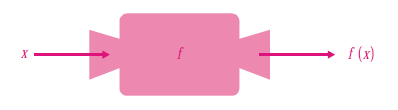
\includegraphics[width=0.8\textwidth]{FunctieMachine}
    \vfill
  \end{center}
  % \vfill
  \vspace*{-2cm}
  \subsection*{Doelstellingen}
  {\singlespacing

    Je kan bijzonderheden van grafieken,
    eventueel aangevuld met tabellen,\\ aflezen zoals: \hfill  {\scriptsize(LP 2005/069, LI 1.1, ET10)}
    \begin{itemize}
    \item het domein,
    \item het bereik, \teacher{het bereik moet niet gekend zijn volgens leerplan}
    \item de nulwaarden,
    \item het stijgen en dalen,
    \item het tekenverloop,
    %\item de periodiciteit,
    \item de symmetrieën,
    \item de extreme waarden
    \end{itemize}
  }


\thispagestyle{empty}
\mbox{}
\newpage
\clearpage
\thispagestyle{empty}
%\mbox{}
\tableofcontents
\newpage
\clearpage
\pagenumbering{arabic} 

\fancyhead[RO,LE]{Reële Functies}
\fancyhead[RE,LO]{}

\onehalfspacing

\pagebreak
\end{theorie}

\section{Reële functie}

\begin{theorie}
\begin{definition}
  Een {\bf reële functie}, of functie in $\mathbb{R}$, is een verzameling van {\em koppels} reële getallen $(x,y)$, zodat elk getal $x$ {\em hoogstens één beeld} $y$ heeft.
\end{definition}

\paragraph{Notatie:} $f$, $g$, $h$, $f_1$, $f_2$, \ldots

Vaak wordt in de notatie expliciet aangegeven dat de functie vertrekt uit de reële getallen en aankomt in de reële getallen:
$$f:\mathbb{R}\to\mathbb{R}$$

\paragraph{Terminologie:}
$$(x,y) \in \mathbb{R}^2$$
\begin{itemize}
  \item $x$ argument, onafhankelijke veranderlijke, abscis, $x$-waarde
  \item $y$ beeld, afhankelijke veranderlijke, ordinaat, $y$-waarde
  \item $\in$ element van
  \item $\mathbb{R}^2$ verzameling van alle koppels reële getallen
\end{itemize}

\end{theorie}

\begin{oefening}
  Geef twee koppels $(x,y)$ waarvan je weet dat ze niet tot dezelfde functie kunnen behoren.
\end{oefening}

\begin{oefening}
\begin{enumerate}[(a)]
  \item Kunnen de koppels $(1,3)$ en $(2,4)$ tot dezelfde functie behoren?
  \item Kunnen de koppels $(1,3)$ en $(1,4)$ tot dezelfde functie behoren?
  \item Kunnen de koppels $(1,3)$ en $(2,3)$ tot dezelfde functie behoren?
  \item Kunnen de koppels $(1,3)$ en $(1,3)$ tot dezelfde functie behoren?
\end{enumerate}
\end{oefening}

\begin{oefening}*
  Beschouw een functie met de naam $f$. De argumenten zijn steeds negatieve reële getallen zonder nul en de beelden zijn steeds positieve reële getallen. Noteer $f$ zo expliciet mogelijk.
\end{oefening}

\pagebreak
\section{Voorstellingswijzen}
\begin{theorie}
We kunnen een functie voorstellen op 3 verschillende manieren. Neem bijvoorbeeld de reële functie die de verzameling van alle koppels $(x,\sqrt{x})$ is.

\paragraph{Functievoorschrift:}
$$f:\mathbb{R}\to\mathbb{R}:x\mapsto\sqrt{x}$$

\paragraph{Functiewaardentabel:}
\begin{center}
  \begin{tabular}{c|cccccccc}
    $x$ & -2 & -1 & 0 & 1 & 2 & 3 & 4\\
    \hline
    $y$ & / & / & 0 & 1 & $1.4$ & $1.7$ & 2\\
  \end{tabular}
\end{center}

\paragraph{Grafiek:}
\begin{center}
  \definecolor{cqcqcq}{rgb}{0.75,0.75,0.75}
  \begin{tikzpicture}[line cap=round,line join=round,>=triangle 45,x=1.0cm,y=1.0cm]
    \draw [color=cqcqcq,dash pattern=on 1pt off 1pt, xstep=1.0cm,ystep=1.0cm] (-1.24,-1.54) grid (9.56,3.5);
    \draw[->,color=black] (-1.24,0) -- (9.56,0);
    \foreach \x in {-1,1,2,3,4,5,6,7,8,9}
    \draw[shift={(\x,0)},color=black] (0pt,2pt) -- (0pt,-2pt) node[below] {\footnotesize $\x$};
    \draw[color=black] (9.24,0.08) node [anchor=south west] {$x$};
    \draw[->,color=black] (0,-1.54) -- (0,3.5);
    \foreach \y in {-1,1,2,3}
    \draw[shift={(0,\y)},color=black] (2pt,0pt) -- (-2pt,0pt) node[left] {\footnotesize $\y$};
    \draw[color=black] (0.1,3.1) node [anchor=west] {$y$};
    \draw[color=black] (0pt,-10pt) node[right] {\footnotesize $0$};
    \clip(-1.24,-1.54) rectangle (9.56,3.5);
    \draw[line width=1.8pt, smooth,samples=500,domain=0:9.56] plot(\x,{sqrt((\x))});
    \draw[color=black] (5,2.6) node[right] {\footnotesize $f$};
    \fill (0,0) circle (2.5pt);
    \fill (1,1) circle (2.5pt);
    \fill (2,1.41) circle (2.5pt);
    \fill (3,1.73) circle (2.5pt);
    \fill (4,2) circle (2.5pt);
  \end{tikzpicture}
\end{center}

We hebben de volgende opmerkingen
\begin{description}
\item[Functievoorschrift:] Dit is de kortste voorstellingswijze. Vaak korten we dit nog als volgt verder in
  $$f(x)=\sqrt{x}$$
  Het voorschrift van een functie kan ook nog geschreven worden als een vergelijking met twee onbekenden, $x$ en $y$. In ons voorbeeld
  $$f: y=\sqrt{x}$$
\item[Functiewaardentabel:] Dit gebruiken we om te helpen bij het tekenen van de grafiek. Hier plaatsen we de koppels $(x,y)$ in een tabel. Weten welke koppels in de tabel moeten komen vraagt een beetje ervaring. Hier hebben we ervoor gekozen om te beginnen bij $-2$ en te eindigen met $4$ en telkens met stapjes van $1$ te verspringen. Een betere keuze was geweest om te beginnen bij $0$ en te eindigen bij $9$. Merk ook op dat we de beelden bij $2$ en $3$ afgerond hebben naar respectievelijk $1.4$ en $1.7$, dit is verantwoord daar we bij het tekenen van de grafiek toch geen grotere nauwkeurigheid kunnen verwachten.
\item[Grafiek:] We beginnen met een orthonormaal assenstelsel te tekenen, dit wil zeggen dat de assen loodrecht op elkaar moeten staan en dat de ijking (de afstand tussen 0 en 1) op elke as gelijk moet zijn. We vergeten niet van de $x$-as en de $y$-as te labelen. Daarna kijken we in de functiewaardentabel. Elk koppel $(x,y)$ die op het assenstelsel past duiden we aan met een punt. De grafiek is dan de vloeiende lijn die de punten verbindt. Merk op dat we de grafiek na het koppel $(4,2)$ blijven verder tekenen. Dit moet ook, want het koppel $(9,3)$ is ook nog een element van de verzameling koppels $(x,\sqrt{x})$.
\end{description}

\end{theorie}

\begin{oefening}
  Schrijf de functie met functievoorschrift
  $$f:\mathbb{R}\to\mathbb{R}:x\mapsto x^2+x+1$$
  nog korter.
\end{oefening}

\begin{oefening}
  Schrijf de volgende functies zo kort mogelijk
  \begin{enumerate}[(a)]
  \itemsep.5em
  \item $f:\mathbb{R}\to\mathbb{R}:x\mapsto \dfrac{1}{x^2+1}$
  \item $f:\mathbb{R}\to\mathbb{R}:x\mapsto 0$
  \item $f:\mathbb{R}\to\mathbb{R}:x\mapsto \sqrt[3]{x^2+1}$
  \item $f:\mathbb{R}\to\mathbb{R}:x\mapsto \left(x^2+1\right)^2$
  \item $f:\mathbb{R}\to\mathbb{R}:x\mapsto x$
  \end{enumerate}
\end{oefening}

\begin{oefening}
  Beschouw de volgende functies en herschrijf ze als een vergelijking van twee onbekenden
  \begin{enumerate}[(a)]
  \itemsep.5em
  \item $f:\mathbb{R}\to\mathbb{R}:x\mapsto \sqrt{5+x^3}$
  \item $f:\mathbb{R}\to\mathbb{R}:x\mapsto 3$
  \item $f:\mathbb{R}\to\mathbb{R}:x\mapsto x$
  \end{enumerate}
\end{oefening}

\begin{oefening}
  Teken met een rode kleur de grafiek van een functie $f$ die door de koppels $(-2, 4)$ en $(2,1)$ gaat. Teken nu met een groene kleur een de grafiek van een andere functie $g$ die door de zelfde koppels gaat.
\end{oefening}

\begin{oefening}
  Welke van de volgende grafieken stellen een functie voor?
  \begin{center}

    \begin{multicols}{2}

      \begin{tikzpicture}[scale=0.2,line cap=round,line join=round,>=triangle 45,x=1.0cm,y=1.0cm]
        \draw[->,color=black] (-10,0) -- (10,0);
        \draw[color=black] (9.68,0.08) node [anchor=south west] { x};
        \draw[->,color=black] (0,-6) -- (0,8);
        \draw[color=black] (0.1,7.6) node [anchor=west] { y};
        \clip(-10,-6) rectangle (10,8);
        \draw [line width=1.6pt,domain=-10.0:0.0] plot(\x,{(-0--2*\x)/-4});
        \draw [line width=1.6pt,domain=0.0:10.0] plot(\x,{(-0--2*\x)/4});
      \end{tikzpicture}

      \begin{tikzpicture}[scale=0.2,line cap=round,line join=round,>=triangle 45,x=1.0cm,y=1.0cm]
        \draw[->,color=black] (-10,0) -- (10,0);
        \draw[color=black] (9.68,0.08) node [anchor=south west] { x};
        \draw[->,color=black] (0,-6) -- (0,8);
        \draw[color=black] (0.1,7.6) node [anchor=west] { y};
        \clip(-10,-6) rectangle (10,8);
        \draw [shift={(0.83,3.84)},line width=1.2pt]  plot[domain=1.01:4.16,variable=\t]({1*2.67*cos(\t r)+0*2.67*sin(\t r)},{0*2.67*cos(\t r)+1*2.67*sin(\t r)});
        \draw [shift={(-10.73,-17.35)},line width=1.2pt]  plot[domain=0.8:1.08,variable=\t]({1*21.47*cos(\t r)+0*21.47*sin(\t r)},{0*21.47*cos(\t r)+1*21.47*sin(\t r)});
        \draw [shift={(3.03,-3.28)},line width=1.2pt]  plot[domain=-1.29:0.84,variable=\t]({1*1.79*cos(\t r)+0*1.79*sin(\t r)},{0*1.79*cos(\t r)+1*1.79*sin(\t r)});
        \draw [shift={(-0.34,11.96)},line width=1.2pt]  plot[domain=4.61:4.94,variable=\t]({1*17.39*cos(\t r)+0*17.39*sin(\t r)},{0*17.39*cos(\t r)+1*17.39*sin(\t r)});
      \end{tikzpicture}

      \begin{tikzpicture}[scale=0.2,line cap=round,line join=round,>=triangle 45,x=1.0cm,y=1.0cm]
        \draw[->,color=black] (-10,0) -- (10,0);
        \draw[color=black] (9.68,0.08) node [anchor=south west] { x};
        \draw[->,color=black] (0,-6) -- (0,8);
        \draw[color=black] (0.1,7.6) node [anchor=west] { y};
        \clip(-10,-6) rectangle (10,8);
        \draw [line width=1.6pt,domain=0.0:10.0] plot(\x,{(--8.01-0.02*\x)/2.86});
        \draw [line width=1.6pt,domain=-10.0:0.0] plot(\x,{(-10.53-1.14*\x)/-3.76});
        \draw [line width=1.6pt,domain=-10.0:0.0] plot(\x,{(-10.08--0.86*\x)/-3.6});
      \end{tikzpicture}

      \begin{tikzpicture}[scale=0.2,line cap=round,line join=round,>=triangle 45,x=1.0cm,y=1.0cm]
        \draw[->,color=black] (-10,0) -- (10,0);
        \draw[color=black] (9.73,0.07) node [anchor=south west] { x};
        \draw[->,color=black] (0,-6) -- (0,8);
        \draw[color=black] (0.09,7.66) node [anchor=west] { y};
        \clip(-10,-6) rectangle (10,8);
        \begin{scriptsize}
          \fill [color=black] (1.46,1.36) circle (4pt);
          \fill [color=black] (2.9,2.6) circle (4pt);
          \fill [color=black] (4.08,3.96) circle (4pt);
          \fill [color=black] (6.2,3.08) circle (4pt);
        \end{scriptsize}
      \end{tikzpicture}

      \begin{tikzpicture}[scale=0.2, line cap=round,line join=round,>=triangle 45,x=1.0cm,y=1.0cm]
        \draw[->,color=black] (-10,0) -- (10,0);
        \draw[color=black] (9.73,0.07) node [anchor=south west] { x};
        \draw[->,color=black] (0,-6) -- (0,8);
        \draw[color=black] (0.09,7.66) node [anchor=west] { y};
        \clip(-10,-6) rectangle (10,8);
        \draw [samples=50,rotate around={-90:(0,0)},xshift=0cm,yshift=0cm,line width=1.6pt] plot (\x,{(\x)^2/2/1.0});
      \end{tikzpicture}

      \begin{tikzpicture}[scale=0.2,line cap=round,line join=round,>=triangle 45,x=1.0cm,y=1.0cm]
        \draw[->,color=black] (-10,0) -- (10,0);
        \draw[color=black] (9.73,0.07) node [anchor=south west] { x};
        \draw[->,color=black] (0,-6) -- (0,8);
        \draw[color=black] (0.09,7.66) node [anchor=west] { y};
        \clip(-10,-6) rectangle (10,8);
        \draw [line width=1.6pt] (3,-6) -- (3,8);
      \end{tikzpicture}

    \end{multicols}

  \end{center}

\end{oefening}


\begin{oefening}
  Welke van onderstaande koppels behoren tot de functie met
  $$f:\mathbb{R}\to\mathbb{R}:x\mapsto\frac{6}{x}$$
  als functievoorschrift?
\end{oefening}
$$(5,-8)\qquad(-1,4)\qquad(2,3)\qquad(\sqrt{2},\frac{2}{3})\qquad(-6,-1)$$

\begin{oefening}
  Geef van een functie met functievoorschrift $f(x)=x^2-4$ een functiewaardentabel die begint bij -5 en eindigt bij 5. Teken daarna de grafiek.
\end{oefening}

\begin{oefening}
  Geef van een functie met functievoorschrift $f(x)=\sqrt{x+4}$ een functiewaardentabel die begint bij -5 en eindigt bij 5. Teken daarna de grafiek.
\end{oefening}

\begin{oefening}*
  Zijn de functies
  $$f(x)=x^2+2x+1$$
  en
  $$g(x)=(x+1)^2$$
  dezelfde of verschillende functies?
\end{oefening}

\begin{oefening}*
  Zijn de functies
  $$f(x)=x^2+4$$
  en
  $$g(x)=(x+2)^2$$
  dezelfde of verschillende functies?
\end{oefening}

\begin{oefening}*
  Zijn de functies
  $$f(x)=x^2-9$$
  en
  $$g(x)=(x+3)(x-3)$$
  dezelfde of verschillende functies?
\end{oefening}


\newpage
\section{Domein en bereik van een functie}

\begin{theorie}
\subsection{Domein}

\begin{definition}
  Het {\bf domein} van een functie is de verzameling van alle $x$-waarden waarvoor de functie een beeld heeft.
\end{definition}

\paragraph{Notatie:} Het domein van de functie $f$ wordt genoteerd als $$\dom f$$ en we lezen dit als {\em domein f}.

\subsubsection{Het domein bepalen aan de hand van het functievoorschrift}

\paragraph{Voorbeeld} Bepaal het domein van $$f:\mathbb{R}\to\mathbb{R}:x\mapsto \sqrt{x}\;.$$

We hebben eerder gezien dat de functie $f(x)=\sqrt{x}$ enkel beelden heeft voor positieve waarden $x$. Zo heeft $x=4$ het beeld $f(4)=\sqrt{4}=2$. Dit wil zeggen dat $4\in\dom f$. Strikt negatieve getallen hebben geen beeld. Zo is $x=-9$ zinloos als argument voor $f$ want $f(-9)=\sqrt{-9}$ bestaat niet. Alle positieve reële getallen kunnen we kort schrijven met de verzameling $\mathbb{R}^+$, we krijgen dus
$$\dom \sqrt{x}= \mathbb{R}^+\;.$$

Opmerking: $0\in\mathbb{R}^+$, dus $0\in\dom\sqrt{x}$. Inderdaad, de $x$-waarde $x=0$ heeft ook een beeld, namelijk $f(0)=\sqrt{0}=0$.

\paragraph{Voorbeeld}
Het domein van
$$f:\mathbb{R}\to\mathbb{R}:x\mapsto 2x+2$$
is
$$\dom 2x+2 = \mathbb{R}\;.$$

Inderdaad, voor elke $x\in\mathbb{R}$ bestaat er een beeld, namelijk $2x+2$. Je kan dus gelijk welk getal kiezen voor $x$, je zal altijd $2x+2$ kunnen uitrekenen. We doen dit eens met een voorbeeld. We nemen willekeurig $x=-8$, dan is $f(-8)=2\cdot(-8)+2=-16+2=-14$. Met andere woorden $-8$ heeft een beeld, namelijk $-14$, en dus is $-8\in\dom f$.

\paragraph{Voorbeeld}
Het domein van
$$f:\mathbb{R}\to\mathbb{R}:x\mapsto \dfrac{1}{x-3}$$
is
$$\dom \dfrac{1}{x-3} = \mathbb{R}\setminus\{3\}\;.$$

Hier zeggen we dus dat het domein van de functie $f$ alle reële getallen zonder $3$ bevat. Het symbool $\setminus$ staat dus voor {\em zonder} en neemt het verschil van twee verzamelingen, in ons geval van alle reële getallen en van de verzameling met enkel het getal $3$. Inderdaad, nemen we $x=3$ en reken we $f(3)$ uit dan krijgen we
$$f(3)=\dfrac{1}{x-3}=\dfrac{1}{3-3}=\dfrac{1}{0}=/$$
omdat we niet kunnen delen door $0$! Eender wel ander getal kunnen we wel kiezen als $x$ en behoort dus wel tot het domein.

\end{theorie}

\begin{oefening}
  Beschouw de functie $\displaystyle f(x)=\dfrac{1}{-3-x}$\\
  \begin{enumerate}[(a)]
  \itemsep.5em
  \item Controleer of $x=-3$ tot het domein van $f$ behoort.
  \item Controleer of $x=3$ tot het domein van $f$ behoort.
  \item Wat is het domein van $f$?
  \end{enumerate}
\end{oefening}

\begin{theorie}
\subsubsection{Het domein bepalen aan de hand van de grafiek}

Het domein bepalen aan de hand van het voorschrift is vaak niet zo eenvoudig. Je moet ofwel alle mogelijke reële getallen proberen, wat praktisch niet haalbaar is omdat $\mathbb{R}$ oneindig veel getallen bevat. Of je moet beredeneren welke getallen wel of niet tot het domein behoren.

Gelukkig bestaat er een veel eenvoudiger methode. Je tekent eerst de grafiek en daarna projecteer je deze grafiek op op de $x$-as. Projecteren op de $x$-as wil zeggen dat we door elk punt van de grafiek een rechte loodrecht tekenen op de $x$-as en dat het geprojecteerde punt dan het snijpunt van deze rechte met de $x$-as is.

Dit lijkt misschien nog steeds moeilijk, maar in de praktijk valt dit best mee. Je gaat als het ware de grafiek van de functie gaan samen drukken op de $x$-as. Alle punten die zo op de $x$-as terecht komen behoren dan tot het domein.

\pagebreak
\paragraph*{Voorbeeld} We bepalen het domein van
$$f:\mathbb{R}\to\mathbb{R}:x\mapsto\sqrt{x+1.5}\;.$$

Binnen het volgende assenstelsel hebben we de volgende stappen ondernomen:
\begin{enumerate}[(1)]
\item We tekenen de grafiek van $f(x)=\sqrt{x+1.5}$. Hiervoor hebben we op een klad blaadje uiteraard eerst een functiewaardentabel gemaakt om te weten door welke punten onze vloeiende lijn moest getekend worden.
\item We projecteren nu elk punt van de grafiek op de $x$-as. Dit is dus de grafiek gewoon samendrukken op de $x$-as.
\item We duiden op de $x$-as nu duidelijk het interval van alle $x$-waarden die een beeld hebben aan met behulp van een dikke lijn.
\end{enumerate}

\begin{center}
  \definecolor{xdxdff}{rgb}{0.49,0.49,1}
  \definecolor{yqyqyq}{rgb}{0.5,0.5,0.5}
  \begin{tikzpicture}[scale=2.25,line cap=round,line join=round,>=triangle 45,x=1.0cm,y=1.0cm]
    \draw[->,color=black] (-2.72,0) -- (3.29,0);
    \foreach \x in {-2.5,-2,-1.5,-1,-0.5,0.5,1,1.5,2,2.5,3}
    \draw[shift={(\x,0)},color=black] (0pt,2pt) -- (0pt,-2pt) node[below] {\footnotesize $\x$};
    \draw[color=black] (3.14,0.04) node [anchor=south west] { x};
    \draw[->,color=black] (0,-0.55) -- (0,2.62);
    \foreach \y in {-0.5,0.5,1,1.5,2,2.5}
    \draw[shift={(0,\y)},color=black] (2pt,0pt) -- (-2pt,0pt) node[left] {\footnotesize $\y$};
    \draw[color=black] (0.05,2.44) node [anchor=west] { y};
    \draw[color=black] (0pt,-10pt) node[right] {\footnotesize $0$};
    \clip(-2.72,-0.55) rectangle (3.29,2.62);
    \draw[line width=1.8pt, smooth,samples=500,domain=-1.5:3.3] plot(\x,{sqrt((\x)+1.5)});
    \draw [->,color=yqyqyq] (-1,0.71) -- (-1,0);
    \draw [->,color=yqyqyq] (0,1.22) -- (0,0);
    \draw [->,color=yqyqyq] (1,1.58) -- (1,0);
    \draw [->,color=yqyqyq] (-0.5,1) -- (-0.5,0);
    \draw [->,color=yqyqyq] (0.5,1.41) -- (0.5,0);
    \draw [->,color=yqyqyq] (1.5,1.73) -- (1.5,0);
    \draw [->,color=yqyqyq] (2.01,1.87) -- (2,0);
    \draw [->,color=yqyqyq] (2.5,2) -- (2.5,0);
    \draw [line width=2.6pt] (4.5,0)-- (-1.5,0);
    \draw (1,2) node[anchor=north west] {(1)};
    \draw (1,0.83) node[anchor=north west] {(2)};
    \draw (1,-0.06) node[anchor=north west] {(3)};
    \begin{scriptsize}
      \fill [color=xdxdff] (4.5,0) circle (1.5pt);
      \draw[color=xdxdff] (4.57,0.12) node {$Q$};
      \fill [color=black] (-1.5,0) circle (1.5pt);
    \end{scriptsize}
  \end{tikzpicture}
\end{center}

We kijken nu op de $x$-as om het domein te bepalen. De kleinste $x$-waarde die tot het domein behoort is $x=-1.5$, er is geen grootste $x$-waarde die tot het domein behoort. We krijgen dus als domein het interval
$$\dom\sqrt{x+1.5}=[-1.5,+\infty[\;.$$

\end{theorie}

\begin{oefening}
  Bepaal grafisch het domein van\\
  \begin{enumerate}[(a)]
    \itemsep.5em
  \item $f:\mathbb{R}\to\mathbb{R}:x\mapsto 2x+2$
  \item $f:\mathbb{R}\to\mathbb{R}:x\mapsto 4-x^2$
  \item $g:\mathbb{R}\to\mathbb{R}:x\mapsto x^3-1$
  \end{enumerate}
\end{oefening}

\begin{oefening}
  Bepaal grafisch het domein van
  $$f:\mathbb{R}\to\mathbb{R}:x\mapsto \dfrac{1}{x-3}\;.$$
  De grafiek van deze functie is de volgende hyperbool
  \begin{center}
    \begin{tikzpicture}[line cap=round,line join=round,>=triangle 45,x=1.0cm,y=1.0cm]
      \draw[->,color=black] (-2.26,0) -- (8.11,0);
      \foreach \x in {-2,-1,1,2,3,4,5,6,7,8}
      \draw[shift={(\x,0)},color=black] (0pt,2pt) -- (0pt,-2pt) node[below] {\footnotesize $\x$};
      \draw[->,color=black] (0,-3.3) -- (0,4.12);
      \foreach \y in {-3,-2,-1,1,2,3,4}
      \draw[shift={(0,\y)},color=black] (2pt,0pt) -- (-2pt,0pt) node[left] {\footnotesize $\y$};
      \draw[color=black] (0pt,-10pt) node[right] {\footnotesize $0$};
      \clip(-2.26,-3.3) rectangle (8.11,4.12);
      \draw[line width=1.8pt, smooth,samples=500,domain=-2.26:2.99] plot(\x,{1/((\x)-3)});
      \draw[line width=1.8pt, smooth,samples=500,domain=3.01:8.1] plot(\x,{1/((\x)-3)});
    \end{tikzpicture}
  \end{center}
\end{oefening}

\begin{oefening}
  Bepaal grafisch het domein van de functie $f$ die bij de volgende grafiek hoort\\
  \begin{center}
    \definecolor{cqcqcq}{rgb}{0.75,0.75,0.75}
    \begin{tikzpicture}[line cap=round,line join=round,>=triangle 45,x=1.0cm,y=1.0cm]
      \draw [color=cqcqcq,dash pattern=on 1pt off 1pt, xstep=1.0cm,ystep=1.0cm] (-3.35,-1.49) grid (6.49,3.26);
      \draw[->,color=black] (-3.35,0) -- (6.49,0);
      \foreach \x in {-3,-2,-1,1,2,3,4,5,6}
      \draw[shift={(\x,0)},color=black] (0pt,2pt) -- (0pt,-2pt) node[below] {\footnotesize $\x$};
      \draw[color=black] (6.2,0.07) node [anchor=south west] {$x$};
      \draw[->,color=black] (0,-1.49) -- (0,3.26);
      \foreach \y in {-1,1,2,3}
      \draw[shift={(0,\y)},color=black] (2pt,0pt) -- (-2pt,0pt) node[left] {\footnotesize $\y$};
      \draw[color=black] (0.09,2.89) node [anchor=west] {$y$};
      \draw[color=black] (0pt,-10pt) node[right] {\footnotesize $0$};
      \clip(-3.35,-1.49) rectangle (6.49,3.26);
      \draw [line width=1.8pt] (-1,1.5)-- (2.9,1.5);
      \draw[color=black] (1.5,1.4) node [anchor=south west] {$f$};
      \begin{scriptsize}
        \fill [color=black] (-1,1.5) circle (2.5pt);
        \draw [color=black] (3,1.5) circle (2.5pt);
      \end{scriptsize}
    \end{tikzpicture}
  \end{center}
\end{oefening}

\begin{theorie}

\subsection{Bereik}

\begin{definition}
  Het {\bf bereik} is de verzameling van alle beelden van een functie.
\end{definition}

\paragraph{Notatie:} Het bereik van de functie $f$ wordt genoteerd als $$\ber f$$ en we lezen dit als {\em bereik f}.

\paragraph{Opmerking:} Men spreekt ook soms van het {\bf beeld} van een functie. Dit staat dus synoniem met het bereik van een functie. Het beeld van een functie is dan dus de verzameling van alle beelden van een functie. De notatie in dit geval is $\mbox{bld }f$.


\subsubsection{Het domein bepalen aan de hand van het functievoorschrift}

\paragraph{Voorbeeld} Bepaal het bereik van $$f:\mathbb{R}\to\mathbb{R}:x\mapsto \sqrt{x+1.5}\;.$$

We herinneren ons dat $\dom f = [-1.5,+\infty[$. De kleinste waarde in het domein is dus $-1.5$. Als we $x=-1.5$ invullen in de functie, krijgen we $f(1.5)=\sqrt{1.5-1.5}=\sqrt{0}=0$. Dus als beeld krijgen we $0$. We vinden alvast dat $0\in\ber f$. Waarden kleiner dan $-1.5$ kunnen we in de functie niet invullen. Laten we een waarde nemen die een klein beetje groter is dan de kleinste waarde uit het domein, bijvoorbeeld $x=-1$. We gebruiken dit nu als argument voor de functie en rekenen uit: $f(-1)=\sqrt{-1+1.5}=\sqrt{0.5}\approx0.71$. We besluiten dus dat $0.71\in\ber f$. We kunnen dus steeds grotere waarden nemen als argument, we merken dat we steeds een positief beeld krijgen. Uiteindelijk kan beredeneerd worden dat
$$\ber \sqrt{x+1.5}=\mathbb{R}^+\;.$$

\subsubsection{Het domein bepalen aan de hand van de grafiek}

Eenvoudig is dit allemaal niet, gelukkig kunnen we het bereik ook snel aflezen met behulp van de grafiek. Aangezien we de beelden zoeken, dus de $y$-waarden, moet er nu geprojecteerd worden op de $y$-as:

\begin{center}
  \definecolor{aqaqaq}{rgb}{0.63,0.63,0.63}
  \begin{tikzpicture}[scale=2.25,line cap=round,line join=round,>=triangle 45,x=1.0cm,y=1.0cm]
    \draw[->,color=black] (-2.65,0) -- (3.24,0);
    \foreach \x in {-2.5,-2,-1.5,-1,-0.5,0.5,1,1.5,2,2.5,3}
    \draw[shift={(\x,0)},color=black] (0pt,2pt) -- (0pt,-2pt) node[below] {\footnotesize $\x$};
    \draw[color=black] (3.09,0.04) node [anchor=south west] { x};
    \draw[->,color=black] (0,-0.65) -- (0,2.59);
    \foreach \y in {-0.5,1.5,2}
    \draw[shift={(0,\y)},color=black] (2pt,0pt) -- (-2pt,0pt) node[left] {\footnotesize $\y$};
    \draw[color=black] (0.05,2.4) node [anchor=west] { y};
    \draw[color=black] (0pt,-10pt) node[right] {\footnotesize $0$};
    \clip(-2.65,-0.65) rectangle (3.24,2.59);
    \draw[line width=1.8pt, smooth,samples=500,domain=-1.5:3.25] plot(\x,{sqrt((\x)+1.5)});
    \draw [->,color=aqaqaq] (-1.25,0.5) -- (0,0.5);
    \draw [->,color=aqaqaq] (-0.5,1) -- (0,1);
    \draw [->,color=aqaqaq] (0.76,1.5) -- (0,1.5);
    \draw [->,color=aqaqaq] (2.5,2) -- (0,2);
    \draw [->,color=aqaqaq] (-1.5,0) -- (0,0);
    \draw [line width=2.6pt] (0,0)-- (0,4.5);
    \fill [color=black] (0,0) circle (1.5pt);
  \end{tikzpicture}
\end{center}

We kijken nu op de $y$-as. De kleinste $y$-waarde is $y=0$, er is geen grootste $y$ waarde, dus het bereik is het interval dat begint bij $0$ en geen einde heeft en we dus noteren met $+\infty$. Dit is dus het interval $[0,+\infty[$ wat we korter kunnen schrijven met $\mathbb{R}^+$:
$$\ber \sqrt{x+1.5}=\mathbb{R}^+\;.$$

\end{theorie}

\begin{oefening}
  Bepaal grafisch het bereik van
  $$f:\mathbb{R}\to\mathbb{R}:x\mapsto \dfrac{1}{x-4}+1\;.$$
  De grafiek van deze functie is de volgende hyperbool
  \begin{center}
    \begin{tikzpicture}[line cap=round,line join=round,>=triangle 45,x=1.0cm,y=1.0cm]
      \draw[->,color=black] (-2.26,0) -- (8.11,0);
      \foreach \x in {-2,-1,1,2,3,4,5,6,7,8}
      \draw[shift={(\x,0)},color=black] (0pt,2pt) -- (0pt,-2pt) node[below] {\footnotesize $\x$};
      \draw[->,color=black] (0,-3.3) -- (0,4.12);
      \foreach \y in {-3,-2,-1,1,2,3,4}
      \draw[shift={(0,\y)},color=black] (2pt,0pt) -- (-2pt,0pt) node[left] {\footnotesize $\y$};
      \draw[color=black] (0pt,-10pt) node[right] {\footnotesize $0$};
      \clip(-2.26,-3.3) rectangle (8.11,4.12);
      \draw[line width=1.8pt, smooth,samples=500,domain=-2.26:3.99] plot(\x,{1/((\x)-4)+1});
      \draw[line width=1.8pt, smooth,samples=500,domain=4.01:8.1] plot(\x,{1/((\x)-4)+1});
    \end{tikzpicture}
  \end{center}
\end{oefening}

\begin{oefening}
  Bepaal grafisch het bereik van
  $$f:\mathbb{R}\to\mathbb{R}:x\mapsto -x^2+6x-7\;.$$
  De grafiek van deze functie is de volgende parabool
  \begin{center}
    \begin{tikzpicture}[line cap=round,line join=round,>=triangle 45,x=1.0cm,y=1.0cm]
      \draw[->,color=black] (-2.26,0) -- (8.11,0);
      \foreach \x in {-2,-1,1,2,3,4,5,6,7,8}
      \draw[shift={(\x,0)},color=black] (0pt,2pt) -- (0pt,-2pt) node[below] {\footnotesize $\x$};
      \draw[->,color=black] (0,-3.3) -- (0,4.12);
      \foreach \y in {-3,-2,-1,1,2,3,4}
      \draw[shift={(0,\y)},color=black] (2pt,0pt) -- (-2pt,0pt) node[left] {\footnotesize $\y$};
      \draw[color=black] (0pt,-10pt) node[right] {\footnotesize $0$};
      \clip(-2.26,-3.3) rectangle (8.11,4.12);
      \draw[line width=1.8pt, smooth,samples=500,domain=-2.26:8.1] plot(\x,{2-(\x-3)^2});
    \end{tikzpicture}
  \end{center}
\end{oefening}

\begin{oefening}
  Bepaal grafisch het bereik van de functie $f$ die bij de volgende grafiek hoort\\
  \begin{center}
    \definecolor{cqcqcq}{rgb}{0.75,0.75,0.75}
    \begin{tikzpicture}[line cap=round,line join=round,>=triangle 45,x=1.0cm,y=1.0cm]
      \draw [color=cqcqcq,dash pattern=on 1pt off 1pt, xstep=1.0cm,ystep=1.0cm] (-3.35,-1.49) grid (6.49,3.26);
      \draw[->,color=black] (-3.35,0) -- (6.49,0);
      \foreach \x in {-3,-2,-1,1,2,3,4,5,6}
      \draw[shift={(\x,0)},color=black] (0pt,2pt) -- (0pt,-2pt) node[below] {\footnotesize $\x$};
      \draw[color=black] (6.2,0.07) node [anchor=south west] {$x$};
      \draw[->,color=black] (0,-1.49) -- (0,3.26);
      \foreach \y in {-1,1,2,3}
      \draw[shift={(0,\y)},color=black] (2pt,0pt) -- (-2pt,0pt) node[left] {\footnotesize $\y$};
      \draw[color=black] (0.09,2.89) node [anchor=west] {$y$};
      \draw[color=black] (0pt,-10pt) node[right] {\footnotesize $0$};
      \clip(-3.35,-1.49) rectangle (6.49,3.26);
      \draw [line width=1.8pt] (-1,1.5)-- (2.9,1.5);
      \draw[color=black] (1.5,1.4) node [anchor=south west] {$f$};
      \begin{scriptsize}
        \fill [color=black] (-1,1.5) circle (2.5pt);
        \draw [color=black] (3,1.5) circle (2.5pt);
      \end{scriptsize}
    \end{tikzpicture}
  \end{center}
\end{oefening}

\begin{oefening}
  Bepaal grafisch het bereik van de functie die bij de volgende grafiek hoort\\
  \begin{center}
    \definecolor{cqcqcq}{rgb}{0.75,0.75,0.75}
    \begin{tikzpicture}[line cap=round,line join=round,>=triangle 45,x=1.0cm,y=1.0cm]
      \draw [color=cqcqcq,dash pattern=on 1pt off 1pt, xstep=1.0cm,ystep=1.0cm] (-3.35,-1.49) grid (6.49,3.26);
      \draw[->,color=black] (-3.35,0) -- (6.49,0);
      \foreach \x in {-3,-2,-1,1,2,3,4,5,6}
      \draw[shift={(\x,0)},color=black] (0pt,2pt) -- (0pt,-2pt) node[below] {\footnotesize $\x$};
      \draw[color=black] (6.2,0.07) node [anchor=south west] {$x$};
      \draw[->,color=black] (0,-1.49) -- (0,3.26);
      \foreach \y in {-1,1,2,3}
      \draw[shift={(0,\y)},color=black] (2pt,0pt) -- (-2pt,0pt) node[left] {\footnotesize $\y$};
      \draw[color=black] (0.09,2.89) node [anchor=west] {$y$};
      \draw[color=black] (0pt,-10pt) node[right] {\footnotesize $0$};
      \clip(-3.35,-1.49) rectangle (6.49,3.26);
      \draw [line width=1.8pt] (-2,2)-- (3,1);
      \begin{scriptsize}
        \fill [color=black] (-2,2) circle (2.5pt);
        \fill [color=black] (3,1) circle (2.5pt);
      \end{scriptsize}
    \end{tikzpicture}
  \end{center}
\end{oefening}


\begin{oefening}
  Teken de grafiek van de functies met onderstaande voorschriften. Bepaal dan het domein en bereik van deze functies:
  \begin{enumerate}[(a)]
    \itemsep0.8em
  \item $\displaystyle f_a : y=2x+15$
  \item $\displaystyle f_b : y=\sqrt{2x}$
  \item $\displaystyle f_c : y=-2x^2+x+1$
  \item $\displaystyle f_d : y=\frac{4}{x^2-25}$
  \item $\displaystyle f_e : y=-5x^2$
  \item $\displaystyle f_f : y=-x^2+2x$
  \item $\displaystyle f_g : y=\sqrt(9-x^2)$
  \item $\displaystyle f_h : y=\sqrt(x^2-4)$
  \end{enumerate}
\end{oefening}

\pagebreak
\section{Nulwaarden}

\begin{theorie}
  
\begin{definition}
  Een {\bf nulwaarde} of {\bf nulpunt} van een functie is een $x$-waarde waarvoor geldt dat het beeld gelijk is aan nul, m.a.w $f(x)=0$.
\end{definition}

\paragraph*{Opmerking:} Een nulwaarde is {\em een} $x$-waarde die moet voldoen aan een bepaalde voorwaarde. Het kan dus best zijn dat er verschillende $x$-waarden zijn die aan deze voorwaarde voldoen. Daarom spreken we in de definitie niet van {\em de} nulwaarde.

\subsection{Algebraïsch}

Een functie kan gezien worden als een vergelijking met twee onbekenden, $x$ en $y$ in $y=f(x)$. Als we de $x$-waarden zoeken waarvoor de beelden gelijk zijn aan $0$ dan kunnen we gewoon $y$ gelijk stellen aan $0$. We krijgen dus $0=f(x)$ wat inderdaad overeenkomt met de definitie.

Praktisch kunnen we het functievoorschrift gelijk stellen aan nul, wegens de definitie $f(x)=0$, dan houden we een vergelijking over met maar één onbekende. Vaak kan deze opgelost worden.

\paragraph{Voorbeeld:} We bepalen algebraïsch de nulwaarde van $f:\mathbb{R}\to\mathbb{R}:x\mapsto-2x+4$:

\begin{itemize}
\item Eerst en vooral herschrijven we het voorschrift $f(x)=-2x+4$
\item We zoeken nu alle $x$-waarden zodat $f(x)=0$
\item Dit is equivalent met $-2x+4=0$
\item Dit lossen we op
  \begin{alignat*}{2}
    && -2x+4 &= 0\\
    \lra &&   -2x &= -4\\
    \lra &&    x &= \dfrac{-4}{-2}\\
    \lra &&    x &= 2\\
    V=\{2\}
  \end{alignat*}
\end{itemize}

We vinden één nulwaarde, namelijk $x_0=2$.

\paragraph*{Opmerking:} Om de verschillende nulwaarden uit elkaar te houden gaan we ze nummeren met een index, dit is een getal dat rechtsonder de $x$ staat. Is er maar één nulwaarde, dan noteren we deze zoals hierboven met $x_0$. Zijn er verschillende nulwaarden, dan nummeren we ze vanaf één. Zijn er bijvoorbeeld drie nulwaarden, dan krijgen we $x_1$, $x_2$ en $x_3$.


\subsection{Grafisch}

\begin{minipage}{0.5\textwidth}
  Is $x_0$ een nulwaarde van een functie $f$, dan geldt dat $f(x_0)=0$. Met andere woorden, dan is het coördinaat $(x_0,0)$ een koppel van de functie $f$.\\

  Alle coördinaten $(x,0)$ met $x\in\mathbb{R}$ liggen op de $x$-as. Meer bepaald ligt ook het coördinaat $(x_0,0)$ op de $x$-as.\\

  We kunnen dus samenvatten:
\end{minipage}
\begin{minipage}{0.5\textwidth}
  \begin{center}
    \begin{tikzpicture}[line cap=round,line join=round,>=triangle 45,x=1.0cm,y=1.0cm]
      \draw[->,color=black] (-1,0) -- (5,0);
      \draw[color=black] (4.83,0.04) node [anchor=south west] { x};
      \draw[->,color=black] (0,-2) -- (0,4);
      \draw[color=black] (0.05,3.78) node [anchor=west] { y};
      \clip(-1,-2) rectangle (5,4);
      \draw[line width=1.8pt, smooth,samples=100,domain=-1.0:5.0] plot(\x,{((\x)-2)*((\x)-6)});
      \fill [color=black] (2,0) circle (3pt);
      \draw[color=black] (2,0.4) node [anchor=west] {$(x_0,0)$};
      \draw[color=black] (1.3,3.5) node [anchor=west] {$f$};
    \end{tikzpicture}
  \end{center}
\end{minipage}

De {\bf nulwaarden} van een functie $f$ zijn alle $x$-waarden van de snijpunten van de grafiek van $f$ met de $x$-as.

\end{theorie}

\begin{oefening}
  Bepaal zowel algebraïsch als grafisch alle nulwaarden van de volgende functies:
  \begin{enumerate}[(a)]
  \itemsep.5em
  \item $f(x)=3x-6$
  \item $f(x)=x-2$
  \item $f(x)=4-x^2$
  \item $f(x)=3x-1x-3+1$
  \end{enumerate}
\end{oefening}

\begin{oefening}
  Bepaal alle nulwaarden van de functie $f$ waarvan de volgende grafiek gegeven is
  \begin{center}
    \begin{tikzpicture}[line cap=round,line join=round,>=triangle 45,x=1.0cm,y=1.0cm]
      \draw[->,color=black] (-5.42,0) -- (5.31,0);
      \foreach \x in {-5,-4,-3,-2,-1,1,2,3,4,5}
      \draw[shift={(\x,0)},color=black] (0pt,2pt) -- (0pt,-2pt) node[below] {\footnotesize $\x$};
      \draw[color=black] (5,0.08) node [anchor=south west] { x};
      \draw[->,color=black] (0,-2.34) -- (0,2.45);
      \foreach \y in {-2,-1,1,2}
      \draw[shift={(0,\y)},color=black] (2pt,0pt) -- (-2pt,0pt) node[left] {\footnotesize $\y$};
      \draw[color=black] (0.1,2.26) node [anchor=west] { y};
      \draw[color=black] (0pt,-10pt) node[right] {\footnotesize $0$};
      \clip(-5.42,-2.34) rectangle (5.31,2.45);
      \draw[line width=1.8pt, smooth,samples=100,domain=-5.4:5.3] plot(\x,{0.2*((\x)+3)*((\x)+1)*((\x)-2)});
      \draw (2.3,1.25) node[anchor=north west] {$f$};
    \end{tikzpicture}
  \end{center}
\end{oefening}

\begin{oefening}
  Bepaal alle nulwaarden van de functie op de volgende grafiek\\
  \begin{center}
    \begin{tikzpicture}[line cap=round,line join=round,>=triangle 45,x=1.0cm,y=1.0cm]
      \draw[->,color=black] (-3.18,0) -- (9.12,0);
      \foreach \x in {-3,-2,-1,1,2,3,4,5,6,7,8,9}
      \draw[shift={(\x,0)},color=black] (0pt,2pt) -- (0pt,-2pt) node[below] {\footnotesize $\x$};
      \draw[->,color=black] (0,-2) -- (0,2.48);
      \foreach \y in {-2,-1,1,2}
      \draw[shift={(0,\y)},color=black] (2pt,0pt) -- (-2pt,0pt) node[left] {\footnotesize $\y$};
      \draw[color=black] (0pt,-10pt) node[right] {\footnotesize $0$};
      \clip(-3.18,-2) rectangle (9.12,2.48);
      \draw [line width=1.8pt, smooth,samples=500,domain=-3:9] plot(\x,{rad(atan(\x-3))});
    \end{tikzpicture}
  \end{center}
\end{oefening}

\begin{oefening}
  Bepaal alle nulwaarden van de functie op de volgende grafiek\\
  \begin{center}
    \begin{tikzpicture}[scale=1.4, line cap=round,line join=round,>=triangle 45,x=1.0cm,y=1.0cm]
      \draw[->,color=black] (-1.9,0) -- (6.28,0);
      \foreach \x in {-1,1,2,3,4,5,6}
      \draw[shift={(\x,0)},color=black] (0pt,2pt) -- (0pt,-2pt) node[below] {\footnotesize $\x$};
      \draw[color=black] (5.96,0.08) node [anchor=south west] { x};
      \draw[->,color=black] (0,-1.56) -- (0,3.38);
      \foreach \y in {-1,1,2,3}
      \draw[shift={(0,\y)},color=black] (2pt,0pt) -- (-2pt,0pt) node[left] {\footnotesize $\y$};
      \draw[color=black] (0.1,2.98) node [anchor=west] { y};
      \draw[color=black] (0pt,-10pt) node[right] {\footnotesize $0$};
      \clip(-1.9,-1.56) rectangle (6.28,3.38);
      \draw[line width=1.8pt, smooth,samples=200,domain=1.5:6.8] plot(\x,{sqrt((\x)-1.5)});
    \end{tikzpicture}
  \end{center}
\end{oefening}

\begin{oefening}
  Bepaal alle nulwaarden van de functie op de volgende grafiek\\
  \begin{center}
    \begin{tikzpicture}[scale=1.4, line cap=round,line join=round,>=triangle 45,x=1.0cm,y=1.0cm]
      \draw[->,color=black] (-1.9,0) -- (6.28,0);
      \foreach \x in {-1,1,2,3,4,5,6}
      \draw[shift={(\x,0)},color=black] (0pt,2pt) -- (0pt,-2pt) node[below] {\footnotesize $\x$};
      \draw[color=black] (5.96,0.08) node [anchor=south west] { x};
      \draw[->,color=black] (0,-1.56) -- (0,3.38);
      \foreach \y in {-1,1,2,3}
      \draw[shift={(0,\y)},color=black] (2pt,0pt) -- (-2pt,0pt) node[left] {\footnotesize $\y$};
      \draw[color=black] (0.1,2.98) node [anchor=west] { y};
      \draw[color=black] (0pt,-10pt) node[right] {\footnotesize $0$};
      \clip(-1.9,-1.56) rectangle (6.28,3.38);
      \draw[line width=1.8pt, smooth,samples=100,domain=-1:4] plot(\x,{(\x-1.3)^4-1});
    \end{tikzpicture}
  \end{center}
\end{oefening}

\newpage
\section{Tekenverloop}

\begin{theorie}

Met het tekenverloop van een functie $f(x)$ bedoelen we dat we nagaan welk teken (positief, negatief of nul) het beeld $y$ heeft als het argument $x$ het domein doorloopt. Een tekenverloop kan overzichtelijk voorgesteld worden in een tabel met de $x$-waarden en het teken van het overeenkomstig beeld.

\subsection{Aflezen van de grafiek}

\paragraph*{Voorbeeld:} We bepalen het tekenverloop van $f: x\mapsto 0.5 x -1.5$

Met behulp van een functiewaardentabel tekenen we eerst de grafiek:

\begin{center}
  \definecolor{cqcqcq}{rgb}{0.75,0.75,0.75}
  \begin{tikzpicture}[line cap=round,line join=round,>=triangle 45,x=1.0cm,y=1.0cm]
    \draw [color=cqcqcq,dash pattern=on 1pt off 1pt, xstep=1.0cm,ystep=1.0cm] (-3.28,-3.34) grid (6.38,2.18);
    \draw[->,color=black] (-3.28,0) -- (6.38,0);
    \foreach \x in {-3,-2,-1,1,2,3,4,5,6}
    \draw[shift={(\x,0)},color=black] (0pt,2pt) -- (0pt,-2pt) node[below] {\footnotesize $\x$};
    \draw[color=black] (6.06,0.08) node [anchor=south west] { x};
    \draw[->,color=black] (0,-3.34) -- (0,2.18);
    \foreach \y in {-3,-2,-1,1,2}
    \draw[shift={(0,\y)},color=black] (2pt,0pt) -- (-2pt,0pt) node[left] {\footnotesize $\y$};
    \draw[color=black] (0.1,1.78) node [anchor=west] { y};
    \draw[color=black] (0pt,-10pt) node[right] {\footnotesize $0$};
    \clip(-3.28,-3.34) rectangle (6.38,2.18);
    \draw[line width=1.6pt, smooth,samples=100,domain=-3.2800000000000002:6.379999999999999] plot(\x,{0.5*(\x)-1.5});
  \end{tikzpicture}
\end{center}

Het tekenverloop plaatsen we in de volgende tabel:

\begin{center}
  \begin{tabular}{c|lcccr}
    $x$ & $-\infty$ & & $3$ & & $+\infty$\\
    \hline
    $f(x)$ & & - & 0 & + &
  \end{tabular}
\end{center}

In de tabel staan bovenaan de $x$-waarden en onderaan de $y$-waarden. Als we van de functie het domein doorlopen van $-\infty$ naar $+\infty$ dan zien we op de grafiek dat in het interval $]-\infty,3[$ op de $x$-as alle beelden onder de $x$-as liggen. Met andere woorden de beelden zijn in dit interval negatief. Dit wordt onderaan in de tabel aangeduid met een $-$. We hebben dat $x_0=3$ een nulwaarde van de functie is, daar is het teken dus nul wat we aanduiden onderaan in de tabel met een $0$. Doorlopen we verder het domein, dan liggen in $]3,+\infty[$ alle beelden boven de $x$-as en zijn ze dus positief, we duiden dit aan met een $+$.

\pagebreak
\subsection{Voorbeelden}

\paragraph{Voorbeeld:} We bepalen nu het tekenverloop van $f:\mathbb{R}\to\mathbb{R}:x\mapsto \dfrac{1}{x-4}+1\;.$

De grafiek van deze functie is de volgende hyperbool
\begin{center}
  \definecolor{cqcqcq}{rgb}{0.75,0.75,0.75}
  \begin{tikzpicture}[line cap=round,scale=0.75,line join=round,>=triangle 45,x=1.0cm,y=1.0cm]
    \draw [color=cqcqcq,dash pattern=on 1pt off 1pt, xstep=1.0cm,ystep=1.0cm] (-2.25,-3.2) grid (8.1,4.2);
    \draw[->,color=black] (-2.26,0) -- (8.11,0);
    \foreach \x in {-2,-1,1,2,3,4,5,6,7,8}
    \draw[shift={(\x,0)},color=black] (0pt,2pt) -- (0pt,-2pt) node[below] {\footnotesize $\x$};
    \draw[->,color=black] (0,-3.3) -- (0,4.12);
    \foreach \y in {-3,-2,-1,1,2,3,4}
    \draw[shift={(0,\y)},color=black] (2pt,0pt) -- (-2pt,0pt) node[left] {\footnotesize $\y$};
    \draw[color=black] (0pt,-10pt) node[right] {\footnotesize $0$};
    \clip(-2.26,-3.3) rectangle (8.11,4.12);
    \draw[line width=1.8pt, smooth,samples=500,domain=-2.26:3.99] plot(\x,{1/((\x)-4)+1});
    \draw[line width=1.8pt, smooth,samples=500,domain=4.01:8.1] plot(\x,{1/((\x)-4)+1});
  \end{tikzpicture}
\end{center}

We doorlopen opnieuw het domein van $]-\infty, +\infty[$. Merk op dat $x=4$ niet in het domein ligt, hier zullen we straks rekening mee moeten houden. We zien dat voor negatieve $x$-waarden het beeld positief is. Het beeld blijft positief tot $x_0=3$ waar we een nulwaarde hebben. Dan is het beeld even negatief tot $x=4$ waar er geen beeld is. Na $x=4$ zal het beeld steeds positief blijven. We krijgen volgend tekenverloop:

\begin{center}
  \begin{tabular}{c|lccccccr}
    $x$ & $-\infty$ & & $3$ & & $4$ & & $+\infty$\\
    \hline
    $f(x)$ & & + & 0 & - & / & + &
  \end{tabular}
\end{center}

\paragraph*{Voorbeeld:} Van de volgende functie krijgen we enkel de grafiek:

\begin{center}
  \definecolor{cqcqcq}{rgb}{0.75,0.75,0.75}
  \begin{tikzpicture}[line cap=round,line join=round,>=triangle 45,x=1.0cm,y=1.0cm]
    \draw [color=cqcqcq,dash pattern=on 1pt off 1pt, xstep=1.0cm,ystep=1.0cm] (-3.35,-1.49) grid (6.49,3.26);
    \draw[->,color=black] (-3.35,0) -- (6.49,0);
    \foreach \x in {-3,-2,-1,1,2,3,4,5,6}
    \draw[shift={(\x,0)},color=black] (0pt,2pt) -- (0pt,-2pt) node[below] {\footnotesize $\x$};
    \draw[color=black] (6.2,0.07) node [anchor=south west] {$x$};
    \draw[->,color=black] (0,-1.49) -- (0,3.26);
    \foreach \y in {-1,1,2,3}
    \draw[shift={(0,\y)},color=black] (2pt,0pt) -- (-2pt,0pt) node[left] {\footnotesize $\y$};
    \draw[color=black] (0.09,2.89) node [anchor=west] {$y$};
    \draw[color=black] (0pt,-10pt) node[right] {\footnotesize $0$};
    \clip(-3.35,-1.49) rectangle (6.49,3.26);
    \draw [line width=1.8pt] (-2,2)-- (1,0);
    \fill [color=black] (-2,2) circle (2.5pt);
    \fill [color=black] (1,0) circle (2.5pt);
    \draw [line width=1.8pt] (2,1)-- (4,2);
    \draw [color=black] (2,1) circle (2.5pt);
    \fill [color=black] (4,2) circle (2.5pt);
  \end{tikzpicture}
\end{center}

Het bijhorende tekenverloop is

\begin{center}
  \begin{tabular}{c|lccccccccccr}
    $x$ & $-\infty$ & & $-2$ & & $1$ & & $2$ & & $4$ & & $+\infty$\\
    \hline
    $y$ & & / & + & + & 0 & / & / & + & + & /
  \end{tabular}
\end{center}

\end{theorie}

\begin{oefening}
  Bepaal het tekenverloop van de functie $f$ uit de volgende grafiek:
  \begin{center}
    \begin{tikzpicture}[line cap=round,line join=round,>=triangle 45,x=1.0cm,y=1.0cm]
      \draw[->,color=black] (-5.42,0) -- (5.31,0);
      \foreach \x in {-5,-4,-3,-2,-1,1,2,3,4,5}
      \draw[shift={(\x,0)},color=black] (0pt,2pt) -- (0pt,-2pt) node[below] {\footnotesize $\x$};
      \draw[color=black] (5,0.08) node [anchor=south west] { x};
      \draw[->,color=black] (0,-2.34) -- (0,2.45);
      \foreach \y in {-2,-1,1,2}
      \draw[shift={(0,\y)},color=black] (2pt,0pt) -- (-2pt,0pt) node[left] {\footnotesize $\y$};
      \draw[color=black] (0.1,2.26) node [anchor=west] { y};
      \draw[color=black] (0pt,-10pt) node[right] {\footnotesize $0$};
      \clip(-5.42,-2.34) rectangle (5.31,2.45);
      \draw[line width=1.8pt, smooth,samples=100,domain=-5.4:5.3] plot(\x,{0.2*((\x)+3)*((\x)+1)*((\x)-2)});
      \draw (2.3,1.25) node[anchor=north west] {$f$};
    \end{tikzpicture}
  \end{center}
\end{oefening}

\begin{oefening}
  Maak de grafiek van de volgende functies en bepaal er dan het tekenverloop van:
  \begin{enumerate}[(a)]
  \item $f(x)=4$
  \item $f(x)=2x-6$
  \item $f(x)=9x^2-4$
  \end{enumerate}
\end{oefening}

\begin{oefening}
  Teken de grafiek van een willekeurige functie en bepaal er dan het tekenverloop van.
\end{oefening}

\begin{oefening}
  Bepaal het tekenverloop van
  \begin{center}
    \definecolor{cqcqcq}{rgb}{0.75,0.75,0.75}
    \begin{tikzpicture}[line cap=round,line join=round,>=triangle 45,x=1.0cm,y=1.0cm]
      \draw [color=cqcqcq,dash pattern=on 1pt off 1pt, xstep=1.0cm,ystep=1.0cm] (-3.35,-2.49) grid (6.49,3.26);
      \draw[->,color=black] (-3.35,0) -- (6.49,0);
      \foreach \x in {-3,-2,-1,1,2,3,4,5,6}
      \draw[shift={(\x,0)},color=black] (0pt,2pt) -- (0pt,-2pt) node[below] {\footnotesize $\x$};
      \draw[color=black] (6.2,0.07) node [anchor=south west] {$x$};
      \draw[->,color=black] (0,-2.49) -- (0,3.26);
      \foreach \y in {-2,-1,1,2,3}
      \draw[shift={(0,\y)},color=black] (2pt,0pt) -- (-2pt,0pt) node[left] {\footnotesize $\y$};
      \draw[color=black] (0.09,2.89) node [anchor=west] {$y$};
      % \draw[color=black] (0pt,-10pt) node[right] {\footnotesize $0$};
      \clip(-3.35,-2.49) rectangle (6.49,3.26);
      \draw [line width=1.8pt] (-2,-1)-- (1,2);
      \fill [color=black] (-2,-1) circle (2.5pt);
      \fill [color=black] (1,2) circle (2.5pt);
      \draw [line width=1.8pt] (2,-2)-- (5,1);
      \fill [color=black] (2,-2) circle (2.5pt);
      \draw [color=black] (5,1) circle (2.5pt);
    \end{tikzpicture}
  \end{center}
\end{oefening}

\pagebreak
\section{Stijgen en dalen}

\subsection{Definities}

\begin{theorie}

\begin{definition}
  De functie $f$ is {\bf stijgend} in een interval $I$ als voor de $x$-waarden $a,b\in I$ met $a<b$ geldt
  $$f(a)\leq f(b)$$
\end{definition}

\begin{definition}
  De functie $f$ is {\bf dalend} in een interval $I$ als voor de $x$-waarden $a,b\in I$ met $a<b$ geldt
  $$f(a)\geq f(b)$$
\end{definition}

\begin{definition}
  Een functie $f$ die zowel stijgend als dalend is in een interval $I$ noemen we {\bf constant} op dat interval $I$.
\end{definition}

\subsection{Voorbeelden}

\paragraph{Voorbeeld:}\mbox{}

\begin{minipage}{0.5\textwidth}
  \begin{center}
    \begin{tikzpicture}[line cap=round,line join=round,>=triangle 45,x=1.0cm,y=1.0cm]
      \draw[->,color=black] (-1,0) -- (6,0);
      \foreach \x in {-1,1,2,3,4,5}
      \draw[shift={(\x,0)},color=black] (0pt,2pt) -- (0pt,-2pt) node[below] {\footnotesize $\x$};
      \draw[color=black] (5.74,0.06) node [anchor=south west] { x};
      \draw[->,color=black] (0,-1) -- (0,4);
      \foreach \y in {-1,1,2,3}
      \draw[shift={(0,\y)},color=black] (2pt,0pt) -- (-2pt,0pt) node[left] {\footnotesize $\y$};
      \draw[color=black] (0.08,3.68) node [anchor=west] { y};
      \draw[color=black] (0pt,-10pt) node[right] {\footnotesize $0$};
      \clip(-1,-1) rectangle (6,4);
      \draw [line width=1.2pt,domain=-1.0:1.0] plot(\x,{(-4-2*\x)/-3});
      \draw [line width=1.2pt] (1,2)-- (3,2);
      \draw [line width=1.2pt,domain=3.0:6.0] plot(\x,{(--16-4*\x)/2});
      \draw [dotted] (1,2)-- (1,0);
      \draw [dotted] (3,2)-- (3,0);
      \begin{scriptsize}
        \fill [color=black] (1,2) circle (2pt);
        \fill [color=black] (3,2) circle (2pt);
      \end{scriptsize}
    \end{tikzpicture}
  \end{center}
\end{minipage}
\begin{minipage}{0.5\textwidth}
  \begin{itemize}
  \item f is {\bf stijgend} in $]-\infty,1]$
  \item f is {\bf constant} in $[1,3]$
  \item f is {\bf dalend} in $[1,+\infty[$
  \end{itemize}
\end{minipage}

\paragraph{Onthoud!} Zoek de $x$-waarden om te bepalen in welk interval de functie stijgend/dalend/constant is.

In de praktijk zullen we de informatie over het stijgend en dalend zijn terug samenvatten in een tabel. Voor bovenstaande voorbeeld wordt dit

\begin{center}
  \begin{tabular}{c|lcccccr}
    $x$ & $-\infty$ & & 1 & & 3 & & $+\infty$\\
    \hline
    $y$ & & $\nearrow$ & & --- & & $\searrow$
  \end{tabular}
\end{center}

In de tabel staan bovenaan de $x$-waarden. In het interval van $]-\infty, 1]$ is de functie stijgend, dit duiden we aan met $\nearrow$. Het interval waar de functie constant is en waar deze dalend is wordt aangeduid met respectievelijk --- en $\searrow$.

Deze tabel wordt het stijgend\&dalend genoemd. Deze tabel zal in het volgende hoofdstuk aangevuld worden met informatie over de maximale en minimale waarden.

\paragraph{Voorbeeld:}

\begin{center}
  \begin{tikzpicture}[line cap=round,line join=round,>=triangle 45,x=1.0cm,y=1.0cm]
    \draw[->,color=black] (-5,0) -- (5,0);
    \foreach \x in {-5,-4,-3,-2,-1,1,2,3,4}
    \draw[shift={(\x,0)},color=black] (0pt,2pt) -- (0pt,-2pt) node[below] {\footnotesize $\x$};
    \draw[color=black] (4.74,0.06) node [anchor=south west] { x};
    \draw[->,color=black] (0,-1) -- (0,4);
    \foreach \y in {-1,1,2,3}
    \draw[shift={(0,\y)},color=black] (2pt,0pt) -- (-2pt,0pt) node[left] {\footnotesize $\y$};
    \draw[color=black] (0.08,3.68) node [anchor=west] { y};
    \draw[color=black] (0pt,-10pt) node[right] {\footnotesize $0$};
    \clip(-5,-1) rectangle (5,4);
    \draw [line width=1.2pt,domain=-5.0:-3.0] plot(\x,{(-12-3*\x)/-1});
    \draw [line width=1.2pt] (-3,3)-- (-1,1);
    \draw [line width=1.2pt] (-1,1)-- (1,3);
    \draw [line width=1.2pt,domain=1.0:5.0] plot(\x,{(--9-3*\x)/2});
    \draw [dotted] (-3,3)-- (-3,0);
    \draw [dotted] (-1,1)-- (-1,0);
    \draw [dotted] (1,3)-- (1,0);
    \begin{scriptsize}
      \fill [color=black] (-3,3) circle (2.0pt);
      \fill [color=black] (-1,1) circle (2.0pt);
      \fill [color=black] (1,3) circle (2.0pt);
      \fill [color=black] (-3,0) circle (2.0pt);
      \fill [color=black] (-1,0) circle (2.0pt);
      \fill [color=black] (1,0) circle (2.0pt);
    \end{scriptsize}
  \end{tikzpicture}
\end{center}

\begin{itemize}
\item f is stijgend in $]-\infty,-3]$ en in $[-1,1]$
\item f is dalend in $[-3,-1]$ en in $[1,+\infty[$
\end{itemize}

Samengevat in het stijgen\&dalen:

\begin{center}
  \begin{tabular}{c|lcccccccr}
    $x$ & $-\infty$ & & -3 & & -1 & & 1 & &$+\infty$\\
    \hline
    $y$ & & $\nearrow$ & & $\searrow$ & & $\nearrow$ & & $\searrow$
  \end{tabular}
\end{center}

\end{theorie}

\begin{oefening}
Bepaal het tekenverloop van de functies die bij de volgende grafieken horen:
    \vspace*{1cm}
    \begin{center}
      \definecolor{cqcqcq}{rgb}{0.75,0.75,0.75}
      \begin{tikzpicture}[scale=0.7,line cap=round,line join=round,>=triangle 45,x=1.0cm,y=1.0cm]
        % \draw [color=cqcqcq,dash pattern=on 1pt off 1pt, xstep=1.0cm,ystep=1.0cm] (-3.28,-3.34) grid (6.38,2.18);
        \draw[->,color=black] (-3.28,0) -- (6.38,0);
        \foreach \x in {-3,-2,-1,1,2,3,4,5,6}
        \draw[shift={(\x,0)},color=black] (0pt,2pt) -- (0pt,-2pt) node[below] {\footnotesize $\x$};
        \draw[color=black] (6.06,0.08) node [anchor=south west] { x};
        \draw[->,color=black] (0,-3.34) -- (0,2.18);
        \foreach \y in {-3,-2,-1,1,2}
        \draw[shift={(0,\y)},color=black] (2pt,0pt) -- (-2pt,0pt) node[left] {\footnotesize $\y$};
        \draw[color=black] (0.1,1.78) node [anchor=west] { y};
        \draw[color=black] (0pt,-10pt) node[right] {\footnotesize $0$};
        \clip(-3.28,-3.34) rectangle (6.38,2.18);
        \draw[line width=1.6pt, smooth,samples=100,domain=-3.2800000000000002:6.379999999999999] plot(\x,{0.5*(\x)-1.5});
      \end{tikzpicture}
    \end{center}
    \vspace*{1cm}
    \begin{center}
      \definecolor{cqcqcq}{rgb}{0.75,0.75,0.75}
      \begin{tikzpicture}[scale=0.7,line cap=round,line join=round,>=triangle 45,x=1.0cm,y=1.0cm]
        % \draw [color=cqcqcq,dash pattern=on 1pt off 1pt, xstep=1.0cm,ystep=1.0cm] (-3.35,-2.49) grid (6.49,3.26);
        \draw[->,color=black] (-3.35,0) -- (6.49,0);
        \foreach \x in {-3,-2,-1,1,2,3,4,5,6}
        \draw[shift={(\x,0)},color=black] (0pt,2pt) -- (0pt,-2pt) node[below] {\footnotesize $\x$};
        \draw[color=black] (6.2,0.07) node [anchor=south west] {$x$};
        \draw[->,color=black] (0,-2.49) -- (0,3.26);
        \foreach \y in {-2,-1,1,2,3}
        \draw[shift={(0,\y)},color=black] (2pt,0pt) -- (-2pt,0pt) node[left] {\footnotesize $\y$};
        \draw[color=black] (0.09,2.89) node [anchor=west] {$y$};
        % \draw[color=black] (0pt,-10pt) node[right] {\footnotesize $0$};
        \clip(-3.35,-2.49) rectangle (6.49,3.26);
        \draw [line width=1.8pt] (-2,-1)-- (1,2);
        \fill [color=black] (-2,-1) circle (2.5pt);
        \fill [color=black] (1,2) circle (2.5pt);
        \draw [line width=1.8pt] (2,-2)-- (5,1);
        \fill [color=black] (2,-2) circle (2.5pt);
        \draw [color=black] (5,1) circle (2.5pt);
      \end{tikzpicture}
    \end{center}
    \vspace*{1cm}
    \begin{center}
      \definecolor{cqcqcq}{rgb}{0.75,0.75,0.75}
      \begin{tikzpicture}[scale=0.7,line cap=round,line join=round,>=triangle 45,x=1.0cm,y=1.0cm]
        % \draw [color=cqcqcq,dash pattern=on 1pt off 1pt, xstep=1.0cm,ystep=1.0cm] (-2.25,-3.2) grid (8.1,4.2);
        \draw[->,color=black] (-2.26,0) -- (8.11,0);
        \foreach \x in {-2,-1,1,2,3,4,5,6,7,8}
        \draw[shift={(\x,0)},color=black] (0pt,2pt) -- (0pt,-2pt) node[below] {\footnotesize $\x$};
        \draw[->,color=black] (0,-3.3) -- (0,4.12);
        \foreach \y in {-3,-2,-1,1,2,3,4}
        \draw[shift={(0,\y)},color=black] (2pt,0pt) -- (-2pt,0pt) node[left] {\footnotesize $\y$};
        \draw[color=black] (0pt,-10pt) node[right] {\footnotesize $0$};
        \clip(-2.26,-3.3) rectangle (8.11,4.12);
        \draw[line width=1.8pt, smooth,samples=500,domain=-2.26:3.99] plot(\x,{1/((\x)-4)+1});
        \draw[line width=1.8pt, smooth,samples=500,domain=4.01:8.1] plot(\x,{1/((\x)-4)+1});
      \end{tikzpicture}
    \end{center}
    \vspace*{1cm}
    \begin{center}
      \begin{tikzpicture}[scale=0.7,line cap=round,line join=round,>=triangle 45,x=1.0cm,y=1.0cm]
        \draw[->,color=black] (-5.42,0) -- (5.31,0);
        \foreach \x in {-5,-4,-3,-2,-1,1,2,3,4,5}
        \draw[shift={(\x,0)},color=black] (0pt,2pt) -- (0pt,-2pt) node[below] {\footnotesize $\x$};
        \draw[color=black] (5,0.08) node [anchor=south west] {$x$};
        \draw[->,color=black] (0,-2.34) -- (0,2.45);
        \foreach \y in {-2,-1,1,2}
        \draw[shift={(0,\y)},color=black] (2pt,0pt) -- (-2pt,0pt) node[left] {\footnotesize $\y$};
        \draw[color=black] (0.1,2.26) node [anchor=west] {$y$};
        \draw[color=black] (0pt,-10pt) node[right] {\footnotesize $0$};
        \clip(-5.42,-2.34) rectangle (5.31,2.45);
        \draw[line width=1.8pt, smooth,samples=100,domain=-5.4:5.3] plot(\x,{0.2*((\x)+3)*((\x)+1)*((\x)-2)});
        \draw (2.3,1.25) node[anchor=north west] {$f$};
      \end{tikzpicture}
    \end{center}
\end{oefening}

\newpage

\section{Extrema}

\begin{theorie}

\subsection{Definities}

De {\bf extrema} van een functie zijn de, eventueel op een klein deel van de functie, grootste of kleinste beelden.

\begin{definition}
  Het reëel getal $m$ is het {\bf minimum} van $f$ op een interval $I$ indien er voor alle $x\in I$ geldt
  $$f(x)\geq m\;.$$
\end{definition}

\begin{definition}
  Het reëel getal $M$ is het {\bf maximum} van $f$ op een interval $I$ indien er voor alle $x\in I$ geldt
  $$f(x)\leq M\;.$$
\end{definition}

Als in de vorige definitie het interval $I$ het volledige domein van de functie $f$ is, dan spreken we van het {\bf absoluut minimum} of {\bf absoluut maximum}. Dit zijn dus respectievelijk de kleinste en de grootste beelden van $f$ op het hele domein.

Indien een functiewaarde maar op een klein deel van het domein het kleinste of grootste beeld is, dan spreken we van een {\bf relatief minimum} of {\bf relatief maximum}.

\subsection{Voorbeeld}

Beschouw de functie waarvan de volgende grafiek wordt gegeven

\begin{center}
  \definecolor{cqcqcq}{rgb}{0.75,0.75,0.75}
  \begin{tikzpicture}[scale=2.0, line cap=round,line join=round,>=triangle 45,x=1.0cm,y=1.0cm]
    \draw [color=cqcqcq,dash pattern=on 1pt off 1pt, xstep=1.0cm,ystep=1.0cm] (-1.27,-1.54) grid (3.48,3.17);
    \draw[->,color=black] (-1.27,0) -- (3.48,0);
    \foreach \x in {-1,1,2,3}
    \draw[shift={(\x,0)},color=black] (0pt,2pt) -- (0pt,-2pt) node[below] {\footnotesize $\x$};
    \draw[color=black] (3.26,0.06) node [anchor=south west] {$x$};
    \draw[->,color=black] (0,-1.54) -- (0,3.17);
    \foreach \y in {-1,1,2,3}
    \draw[shift={(0,\y)},color=black] (2pt,0pt) -- (-2pt,0pt) node[left] {\footnotesize $\y$};
    \draw[color=black] (0.07,2.9) node [anchor=west] {$y$};
    \draw[color=black] (0pt,-10pt) node[right] {\footnotesize $0$};
    \clip(-1.27,-1.54) rectangle (3.48,3.17);
    \draw[line width=1.6pt, smooth,samples=100,domain=-1.2712156348070227:3.4799703926684455] plot(\x,{2*(\x)^3-9*(\x)^2+12*(\x)-3});
    \draw (2.68,1.79) node[anchor=north west] {$f$};
  \end{tikzpicture}
\end{center}

Als we inzoomen op het interval $[0.5,1.5]$ dan merken we dat dit interval bij $x=1$ een grootste functiewaarde heeft, namelijk $f(1)=2$. $y=2$ is dus een maximum in $[0.5,1.5]$. Dit maximum is niet het grootste beeld van de functie want het bereik van de functie is $\ber f=\mathbb{R}$. Dit maximum is dus wel een relatief maximum van de functie, de waarde van het relatief maximum is $y=2$. Analoog vinden we een relatief minimum $y=1$ bij $x=2$. We vatten dit samen in het stijgen\&dalen:

\begin{center}
  \begin{tabular}{c|lcccccr}
    $x$ & $-\infty$ & & 1 & & 2 & & $+\infty$\\
    \hline
    $y$ & & $\nearrow$ & $\underset{=2}{\max}$ & $\searrow$ & $\underset{=1}{\min}$ & $\nearrow$
  \end{tabular}
\end{center}

\paragraph{Onthoud!} Zoek de $y$-waarden om te bepalen waar de functie een minimum/maximum bereikt.

\end{theorie}

\begin{oefening}
Bepaal alle extrema van de volgende grafieken.
    \vspace*{1cm}
    \begin{center}
      \definecolor{cqcqcq}{rgb}{0.75,0.75,0.75}
      \begin{tikzpicture}[scale=0.7,line cap=round,line join=round,>=triangle 45,x=1.0cm,y=1.0cm]
        \draw [color=cqcqcq,dash pattern=on 1pt off 1pt, xstep=1.0cm,ystep=1.0cm] (-3.35,-2.49) grid (6.49,3.26);
        \draw[->,color=black] (-3.35,0) -- (6.49,0);
        \foreach \x in {-3,-2,-1,1,2,3,4,5,6}
        \draw[shift={(\x,0)},color=black] (0pt,2pt) -- (0pt,-2pt) node[below] {\footnotesize $\x$};
        \draw[color=black] (6.2,0.07) node [anchor=south west] {$x$};
        \draw[->,color=black] (0,-2.49) -- (0,3.26);
        \foreach \y in {-2,-1,1,2,3}
        \draw[shift={(0,\y)},color=black] (2pt,0pt) -- (-2pt,0pt) node[left] {\footnotesize $\y$};
        \draw[color=black] (0.09,2.89) node [anchor=west] {$y$};
        \clip(-3.35,-2.49) rectangle (6.49,3.26);
        \draw [line width=1.8pt] (-2,-1)-- (5,1);
        \fill [color=black] (-2,-1) circle (2.5pt);
        \draw [color=black] (5,1) circle (2.5pt);
      \end{tikzpicture}
    \end{center}
    \vspace*{1cm}
    \begin{center}
      \definecolor{cqcqcq}{rgb}{0.75,0.75,0.75}
      \begin{tikzpicture}[scale=0.7,line cap=round,line join=round,>=triangle 45,x=1.0cm,y=1.0cm]
        \draw [color=cqcqcq,dash pattern=on 1pt off 1pt, xstep=1.0cm,ystep=1.0cm] (-2.25,-3.2) grid (8.1,4.2);
        \draw[->,color=black] (-2.26,0) -- (8.11,0);
        \foreach \x in {-2,-1,1,2,3,4,5,6,7,8}
        \draw[shift={(\x,0)},color=black] (0pt,2pt) -- (0pt,-2pt) node[below] {\footnotesize $\x$};
        \draw[->,color=black] (0,-3.3) -- (0,4.12);
        \foreach \y in {-3,-2,-1,1,2,3,4}
        \draw[shift={(0,\y)},color=black] (2pt,0pt) -- (-2pt,0pt) node[left] {\footnotesize $\y$};
        \draw[color=black] (0pt,-10pt) node[right] {\footnotesize $0$};
        \clip(-2.26,-3.3) rectangle (8.11,4.12);
        \draw[line width=1.8pt, smooth,samples=500,domain=-2.26:3.99] plot(\x,{1/((\x)-4)+1});
        \draw[line width=1.8pt, smooth,samples=500,domain=4.01:8.1] plot(\x,{1/((\x)-4)+1});
      \end{tikzpicture}
    \end{center}
    \vspace*{1cm}
    \begin{center}
      \definecolor{cqcqcq}{rgb}{0.75,0.75,0.75}
      \begin{tikzpicture}[scale=0.7,line cap=round,line join=round,>=triangle 45,x=1.0cm,y=1.0cm]
        \draw [color=cqcqcq,dash pattern=on 1pt off 1pt, xstep=1.0cm,ystep=1.0cm] (-5.1,-2.1) grid (5.1,2.1);
        \draw[->,color=black] (-5.42,0) -- (5.31,0);
        \foreach \x in {-5,-4,-3,-2,-1,1,2,3,4,5}
        \draw[shift={(\x,0)},color=black] (0pt,2pt) -- (0pt,-2pt) node[below] {\footnotesize $\x$};
        \draw[color=black] (5,0.08) node [anchor=south west] {$x$};
        \draw[->,color=black] (0,-2.34) -- (0,2.45);
        \foreach \y in {-2,-1,1,2}
        \draw[shift={(0,\y)},color=black] (2pt,0pt) -- (-2pt,0pt) node[left] {\footnotesize $\y$};
        \draw[color=black] (0.1,2.26) node [anchor=west] {$y$};
        \draw[color=black] (0pt,-10pt) node[right] {\footnotesize $0$};
        \clip(-5.42,-2.34) rectangle (5.31,2.45);
        \draw[line width=1.8pt, smooth,samples=100,domain=-5.4:5.3] plot(\x,{0.2*((\x)+3)*((\x)+1)*((\x)-2)});
        \draw (2.3,1.25) node[anchor=north west] {$f$};
      \end{tikzpicture}
    \end{center}
\end{oefening}

\pagebreak

\section{Symmetrie}

\begin{theorie}

Een functie $f$ kan een {\bf lijnsymmetrie} of een {\bf puntsymmetrie} hebben. In het eerste geval is er een rechte, de {\bf as van symmetrie} genoemd waarrond we de grafiek van de functie kunnen spiegelen zonder dat grafiek zal veranderen. In het tweede geval is er een punt waarrond we de grafiek kunnen spiegelen, namelijk {\bf punt van symmetrie} waarrond we de grafiek kunnen spiegelen. Een functie kan meer dan één lijn- en/of puntsymmetrie hebben.

\subsection{Lijnsymmetrie}

Als een functie een as van symmetrie heeft, dan zal het meestal een verticale zijn. Stel dat het een horizontale as zou zijn en we spiegelen daar een punt van de de grafiek rond, dan zouden we twee $y$-waarden moeten hebben zodat de grafiek symmetrisch zou zijn. Maar een functie kan hoogstens één $y$-waarde per $x$-waarde hebben.

We zoeken dus een rechte $x=p$. En we weten dat als we een afstand $a$ naar rechts gaan, dat we het beeld daar moeten kunnen spiegelen op een afstand $a$ naar links. Dit betekend dus voor de functie $f$ die symmetrisch is rond $x=p$ dat er geldt
$$f(p-a)=f(p+a)\qquad\forall a\in \dom f$$

\subsubsection*{Voorbeeld}

We nemen bijvoorbeeld de functie $f(x)=x^2-4x+3$
\begin{center}
\begin{tikzpicture}[line cap=round,line join=round,>=triangle 45,x=1.0cm,y=1.0cm]
\draw[->,color=black] (-2.24,0) -- (6.4,0);
\foreach \x in {-2,-1,1,2,3,4,5,6}
\draw[shift={(\x,0)},color=black] (0pt,2pt) -- (0pt,-2pt) node[below] {\footnotesize $\x$};
\draw[->,color=black] (0,-1.44) -- (0,5.1);
\foreach \y in {-1,1,2,3,4,5}
\draw[shift={(0,\y)},color=black] (2pt,0pt) -- (-2pt,0pt) node[left] {\footnotesize $\y$};
\draw[color=black] (0pt,-10pt) node[right] {\footnotesize $0$};
\clip(-2.24,-1.44) rectangle (6.4,5.1);
\draw[line width=1.8pt, smooth,samples=100,domain=-2.24:6.4] plot(\x,{(\x)^2-4*(\x)+3});
\draw [dotted, line width=1.2pt] (2,-1.44) -- (2,5.1);
\draw (2.26,3.58) node[anchor=north west] {$x=2$};
\draw (2.28,-0.6) node[anchor=north west] {$f(x)=x^2-4x+3$};
\end{tikzpicture}
\end{center}

Grafisch kunnen we de as van symmetrie bepalen met onze geodriehoek, deze is
$$x=2$$.

Algebraïsch kunnen we bovenstaande identiteit gebruiken, hier is $p=2$ en we tonen aan dat $f(2-a)=f(2+a)$ voor een willekeurige $a$:
\begin{eqnarray*}
  f(2-a) &=& (2-a)^2-4(2-a)+3\\
         &=& 4-4a+a^2-8+4a+3\\
         &=& a^2-1
\end{eqnarray*}
en
\begin{eqnarray*}
  f(2+a) &=& (2+a)^2-4(2+a)+3\\
         &=& 4+4a+a^2-8-4a+3\\
         &=& a^2-1
\end{eqnarray*}

\subsection{Puntsymmetrie}

Als een functie symmetrisch is ten opzichte van het punt $(p,q)$, dan wil dat zeggen dat als we een afstand $a$ naar rechts gaan dat dan de gespiegelde $y$-waarde even ver (omhoog of omlaag) van $q$ moet liggen. Dus het gemiddelde van de $y$-waarden moet gelijk zijn aan $q$, dus er geldt
$$\dfrac{f(p-a)+f(p+a)}{2}=q \qquad \forall a\in\dom f$$

\subsubsection*{Voorbeeld}

We nemen bijvoorbeeld de functie $f(x)=0.5x+1$.

\begin{center}
\begin{tikzpicture}[line cap=round,line join=round,>=triangle 45,x=1.0cm,y=1.0cm]
\draw[->,color=black] (-1.14,0) -- (6.5,0);
\foreach \x in {-1,1,2,3,4,5,6}
\draw[shift={(\x,0)},color=black] (0pt,2pt) -- (0pt,-2pt) node[below] {\footnotesize $\x$};
\draw[->,color=black] (0,-1.24) -- (0,4.4);
\foreach \y in {-1,1,2,3,4}
\draw[shift={(0,\y)},color=black] (2pt,0pt) -- (-2pt,0pt) node[left] {\footnotesize $\y$};
\draw[color=black] (0pt,-10pt) node[right] {\footnotesize $0$};
\clip(-1.14,-1.24) rectangle (6.5,4.4);
\draw[line width=1.2pt, smooth,samples=100,domain=-1.1400000000000001:6.5] plot(\x,{0.5*(\x)+1});
\draw (1.2,1.6) node[anchor=north west] {$f(x)=0.5x+1$};
\draw (4.06,2.94) node[anchor=north west] {$(4,3)$};
\begin{scriptsize}
\fill (4,3) circle (1.8pt);
\end{scriptsize}
\end{tikzpicture}
\end{center}

Aan de grafiek zien we dat elk punt op die rechte een punt van symmetrie heeft. We merken ook op dat elke rechte loodrecht op die grafiek een as van symmetrie heeft. Deze rechte heeft dus een oneindig aantal symmetrieën.

We tonen eens algebraïsch aan dat het punt $(4,3)$ op de rechte inderdaad een punt van symmetrie is. We gebruiken dus $p=4$ en $q=3$ in bovenstaande identiteit en moeten dus aantonen dat $\dfrac{f(4-a)+f(4+a)}{2}=3$ voor een willekeurig $a$:
\begin{eqnarray*}
  \dfrac{f(4-a)+f(4+a)}{2} &=& \dfrac{0.5(4-a)+1 + 0.5(4+a)+1}{2}\\
                           &=& \dfrac{2-0.5a + 1 + 2+0.5a + 1}{2}\\
                           &=& \dfrac{6}{2}\\
                           &=& 3
\end{eqnarray*}

\end{theorie}

\begin{oefening}
Beschouw de grafiek van een functie $f$.
\begin{center}
  \definecolor{cqcqcq}{rgb}{0.75,0.75,0.75}
  \begin{tikzpicture}[scale=1.2,line cap=round,line join=round,>=triangle 45,x=1.0cm,y=1.0cm]
    % \draw [color=cqcqcq,dash pattern=on 1pt off 1pt, xstep=1.0cm,ystep=1.0cm] (-3.28,-3.34) grid (6.38,2.18);
    \draw[->,color=black] (-3.28,0) -- (6.38,0);
    \foreach \x in {-3,-2,-1,1,2,3,4,5,6}
    \draw[shift={(\x,0)},color=black] (0pt,2pt) -- (0pt,-2pt) node[below] {\footnotesize $\x$};
    \draw[color=black] (6.06,0.08) node [anchor=south west] {$x$};
    \draw[->,color=black] (0,-3.34) -- (0,2.18);
    \foreach \y in {-3,-2,-1,1,2}
    \draw[shift={(0,\y)},color=black] (2pt,0pt) -- (-2pt,0pt) node[left] {\footnotesize $\y$};
    \draw[color=black] (0.1,1.8) node [anchor=west] {$y$};
    \draw[color=black] (0pt,-10pt) node[right] {\footnotesize $0$};
    \clip(-3.28,-3.34) rectangle (6.38,2.18);
    \draw[line width=1.6pt, smooth,samples=100,domain=-3.28:6.38] plot(\x,{0.5*(\x)-1.5});
    \draw[color=black] (4,1) node[right] {\footnotesize $f$};
  \end{tikzpicture}
\end{center}
\begin{enumerate}[(a)]
  \item Duid een lijnsymmetrie aan op de grafiek.
  \item Zijn er nog andere lijnsymmetrieën?
  \item Duid een puntsymmetrie aan op de grafiek.
  \item Zijn er nog andere puntsymmetrieën?
\end{enumerate}
\end{oefening}

\begin{oefening}
Beschouw de grafiek van een functie $f$.
\begin{center}
      \definecolor{cqcqcq}{rgb}{0.75,0.75,0.75}
      \begin{tikzpicture}[scale=1.2,line cap=round,line join=round,>=triangle 45,x=1.0cm,y=1.0cm]
        % \draw [color=cqcqcq,dash pattern=on 1pt off 1pt, xstep=1.0cm,ystep=1.0cm] (-2.25,-3.2) grid (8.1,4.2);
        \draw[->,color=black] (-2.26,0) -- (8.11,0);
        \foreach \x in {-2,-1,1,2,3,4,5,6,7,8}
        \draw[shift={(\x,0)},color=black] (0pt,2pt) -- (0pt,-2pt) node[below] {\footnotesize $\x$};
        \draw[->,color=black] (0,-3.3) -- (0,4.12);
        \foreach \y in {-3,-2,-1,1,2,3,4}
        \draw[shift={(0,\y)},color=black] (2pt,0pt) -- (-2pt,0pt) node[left] {\footnotesize $\y$};
        \draw[color=black] (0pt,-10pt) node[right] {\footnotesize $0$};
        \clip(-2.26,-3.3) rectangle (8.11,4.12);
        \draw[line width=1.8pt, smooth,samples=500,domain=-2.26:3.99] plot(\x,{1/((\x)-4)+1});
        \draw[line width=1.8pt, smooth,samples=500,domain=4.01:8.1] plot(\x,{1/((\x)-4)+1});
      \end{tikzpicture}
\end{center}
\begin{enumerate}[(a)]
  \item Duid een lijnsymmetrie aan op de grafiek.
  \item Zijn er nog andere lijnsymmetrieën?
  \item Duid een puntsymmetrie aan op de grafiek.
  \item Zijn er nog andere puntsymmetrieën?
\end{enumerate}
\end{oefening}

\begin{oefening}
Beschouw de grafiek van een functie $f$.
\begin{center}
  \definecolor{cqcqcq}{rgb}{0.75,0.75,0.75}
      \begin{tikzpicture}[scale=1.2,line cap=round,line join=round,>=triangle 45,x=1.0cm,y=1.0cm]
        \draw[->,color=black] (-5.42,0) -- (5.31,0);
        \foreach \x in {-5,-4,-3,-2,-1,1,2,3,4,5}
        \draw[shift={(\x,0)},color=black] (0pt,2pt) -- (0pt,-2pt) node[below] {\footnotesize $\x$};
        \draw[color=black] (5,0.08) node [anchor=south west] {$x$};
        \draw[->,color=black] (0,-2.34) -- (0,2.45);
        \foreach \y in {-2,-1,1,2}
        \draw[shift={(0,\y)},color=black] (2pt,0pt) -- (-2pt,0pt) node[left] {\footnotesize $\y$};
        \draw[color=black] (0.1,2.26) node [anchor=west] {$y$};
        \draw[color=black] (0pt,-10pt) node[right] {\footnotesize $0$};
        \clip(-5.42,-2.34) rectangle (5.31,2.45);
        \draw[line width=1.8pt, smooth,samples=100,domain=-5.4:5.3] plot(\x,{0.2*((\x)+3)*((\x)+1)*((\x)-2)});
        \draw (2.3,1.25) node[anchor=north west] {$f$};
      \end{tikzpicture}
\end{center}
\begin{enumerate}[(a)]
  \item Duid een lijnsymmetrie aan op de grafiek.
  \item Zijn er nog andere lijnsymmetrieën?
  \item Duid een puntsymmetrie aan op de grafiek.
  \item Zijn er nog andere puntsymmetrieën?
\end{enumerate}
\end{oefening}

\begin{oefening}
Beschouw de functie
$$f(x)=-x^2+9x-18$$
\begin{enumerate}[(a)]
  \item Teken de grafiek.
  \item Teken de as van symmetrie.
  \item Wat is de vergelijking $x=p$ van de as van symmetrie?
  \item Toon aan dat het punt (2,-4) op de grafiek van $f$ ligt.
  \item Op welk punt spiegelt de as van symmetrie dat punt?
  \item Toon dit ook algebraïsch aan m.b.v. de formule
  $$f(p-a)=f(p+a)$$
\end{enumerate}
\end{oefening}

\begin{oefening}
De functie 
$$f(x)=x^3-9x^2+6x+56$$
heeft één punt van symmetrie, namelijk
$$(p,q)=(3,20)$$
Gebruik de formule
$$\dfrac{f(p-a)+f(p+a)}{2}=q$$
met drie zelf gekozen waarden voor de afstand $a$ om aan te tonen dat de functie inderdaad symmetrisch is rond dat punt.
\end{oefening}


\pagebreak

\section{Extra oefeningen}

\begin{oefening}
  Bepaal voor onderstaande functie
  \begin{center}
    \begin{tikzpicture}[scale=0.7,line cap=round,line join=round,>=triangle 45,x=1.0cm,y=1.0cm]
      \draw[->,color=black] (-7,0) -- (11,0);
      \foreach \x in {-7,-6,-5,-4,-3,-2,-1,1,2,3,4,5,6,7,8,9,10}
      \draw[shift={(\x,0)},color=black] (0pt,2pt) -- (0pt,-2pt) node[below] {\footnotesize $\x$};
      \draw[->,color=black] (0,-4) -- (0,7);
      \foreach \y in {-4,-3,-2,-1,1,2,3,4,5,6}
      \draw[shift={(0,\y)},color=black] (2pt,0pt) -- (-2pt,0pt) node[left] {\footnotesize $\y$};
      \draw[color=black] (0pt,-10pt) node[right] {\footnotesize $0$};
      \clip(-7,-4) rectangle (11,7);
      \draw [line width=1.6pt,domain=-7.0:-6.0] plot(\x,{(-6-1*\x)/-1});
      \draw [line width=1.6pt,domain=9.0:11.0] plot(\x,{(--3-1*\x)/2});
      \draw [line width=1.2pt] (-6,0)-- (-5,3);
      \draw [line width=1.2pt] (-5,3)-- (-3,0);
      \draw [line width=1.2pt] (-3,0)-- (0,-2);
      \draw [line width=1.2pt] (0,-2)-- (2,0);
      \draw [line width=1.2pt] (2,0)-- (5,6);
      \draw [line width=1.2pt] (5,6)-- (7,0);
      \draw [line width=1.2pt] (7,0)-- (9,-3);
    \end{tikzpicture}
  \end{center}

  \begin{itemize}
  \item het domein
  \item het bereik
  \item de nulwaarden
  \item de coördinaten van de snijpunten met de $x$-as
  \item de coördinaten van de snijpunten met de $y$-as
  \item in welke intervallen de functie stijgend is
  \item in welke intervallen de functie dalend is
  \item de minima
  \item de maxima
  \end{itemize}
\end{oefening}


\begin{oefening}
  Gebruik de grafiek om het domein, het bereik, de nulwaarde(n), het tekenverloop, het stijgen \& dalen, de extrema en de symmetrieën te bepalen.

  $$f(x):\;x\mapsto y=\frac{15}{x^2+3}$$

  \begin{center}
    \begin{tikzpicture}[line cap=round,line join=round,>=triangle 45,x=1.0cm,y=1.0cm]
      \draw[->,color=black] (-5,0) -- (5,0);
      \foreach \x in {-4,-2,2,4}
      \draw[shift={(\x,0)},color=black] (0pt,2pt) -- (0pt,-2pt) node[below] {\footnotesize $\x$};
      \draw[->,color=black] (0,-1) -- (0,6.5);
      \foreach \y in {,2,4,6}
      \draw[shift={(0,\y)},color=black] (2pt,0pt) -- (-2pt,0pt) node[left] {\footnotesize $\y$};
      \draw[color=black] (0pt,-10pt) node[right] {\footnotesize $0$};
      \clip(-5,-1) rectangle (5,6.5);
      \draw[line width=1.6pt, smooth,samples=100,domain=-5.0:5.0] plot(\x,{15/((\x)^2+3)});
      \draw (1.26,4.62) node[anchor=north west] {$ f(x)=\frac{15}{x^2+3} $};
    \end{tikzpicture}
  \end{center}

\end{oefening}


\begin{oefening}
  Gebruik de grafiek om het domein, het bereik, de nulwaarde(n), het tekenverloop, het stijgen \& dalen, de extrema en de symmetrieën te bepalen.

  $$f(x):\;x\mapsto y=x^3+3x^2+2$$

  \begin{center}
    \begin{tikzpicture}[line cap=round,line join=round,>=triangle 45,x=1.0cm,y=1.0cm]
      \draw[->,color=black] (-5,0) -- (5,0);
      \foreach \x in {-4,-2,2,4}
      \draw[shift={(\x,0)},color=black] (0pt,2pt) -- (0pt,-2pt) node[below] {\footnotesize $\x$};
      \draw[->,color=black] (0,-1) -- (0,7);
      \foreach \y in {,2,4,6}
      \draw[shift={(0,\y)},color=black] (2pt,0pt) -- (-2pt,0pt) node[left] {\footnotesize $\y$};
      \draw[color=black] (0pt,-10pt) node[right] {\footnotesize $0$};
      \clip(-5,-1) rectangle (5,7);
      \draw[line width=1.6pt, smooth,samples=100,domain=-5.0:5.0] plot(\x,{(\x)^3+3*(\x)^2+2});
      \draw (-3,6) node[anchor=north west] {$ f $};
    \end{tikzpicture}
  \end{center}

\end{oefening}

\begin{oefening}
  Gebruik de grafiek om het domein, het bereik, de nulwaarde(n), het tekenverloop, het stijgen \& dalen, de extrema en de symmetrieën te bepalen.

  $$f(x)=\sqrt{9-x^2}$$

  \begin{center}
    \begin{tikzpicture}[line cap=round,line join=round,>=triangle 45,x=1.0cm,y=1.0cm]
      \draw[->,color=black] (-5,0) -- (5,0);
      \foreach \x in {-4,-2,2,4}
      \draw[shift={(\x,0)},color=black] (0pt,2pt) -- (0pt,-2pt) node[below] {\footnotesize $\x$};
      \draw[->,color=black] (0,-1) -- (0,5);
      \foreach \y in {,2,4}
      \draw[shift={(0,\y)},color=black] (2pt,0pt) -- (-2pt,0pt) node[left] {\footnotesize $\y$};
      \draw[color=black] (0pt,-10pt) node[right] {\footnotesize $0$};
      \clip(-5,-1) rectangle (5,5);
      \draw[line width=1.6pt, smooth,samples=100,domain=-3:3] plot(\x,{(9-(\x)^2)^(1/2)});
      \draw (-3,6) node[anchor=north west] {$ f $};
    \end{tikzpicture}
  \end{center}

\end{oefening}

\begin{oefening}
  Teken de grafiek van de volgende functies en bepaal het domein, het bereik, de nulwaarde(n), het tekenverloop, het stijgen \& dalen, de extrema en de symmetrieën.
  \begin{enumerate}[(a)]
    \itemsep.5em
    \item $f(x)=2x$
    \item $f(x)=-2$
    \item $f(x)=(x-2)^2-4$
    \item $f(x)=(x-2)^3-4$
    \item $f(x)=\sqrt{x-2}-4$
  \end{enumerate}

\end{oefening}


\end{document}
